\documentclass[letterpaper,12pt]{article}
\usepackage{amsmath}
\usepackage{amsthm}              % See geometry.pdf to learn the layout options. There are lots.
\usepackage{geometry}
\usepackage[figuresleft]{rotating}
\usepackage{pdflscape}
%\geometry{a5paper}                   % ... or a4paper or a5paper or ...
%\geometry{landscape}                % Activate for for rotated page geometry
%\usepackage[parfill]{parskip}    % Activate to begin paragraphs with an empty line rather than an indent
\usepackage{afterpage}
\usepackage{graphicx}
\usepackage{amssymb}
\usepackage{epstopdf}
\usepackage{multirow}
\usepackage{booktabs}
\usepackage{setspace}
\usepackage{float}
\setlength{\columnseprule}{.4pt}
%\doublespacing
\usepackage{natbib} % if you're using natbib
\setlength{\bibsep}{0pt} % removes the space between items
\usepackage[multiple]{footmisc}
\geometry{left=1in,right=1in,top=1in,bottom=1in}
%\makeatother \addtolength{\textwidth}{0.4in}
%\addtolength{\oddsidemargin}{-0.2in}
%\addtolength{\textheight}{0.8in} \addtolength{\topmargin}{-0.4in}
\newtheorem{prop}{Proposition}
\newtheorem{cor}{Corollary}
\newtheorem{lemma}{Lemma}
\newtheorem{assumption}{Assumption}
\usepackage{xcolor}
\setlength{\tabcolsep}{2pt}
\usepackage{xr}
 \externaldocument{Paper}

% datatool to  make ces in Latex to external values
\usepackage{datatool}
\DTLsetseparator{|}
\DTLloaddb{valuesData}{Sections/valuesDataUpdated.csv}
%\DTLloaddb{valuesData2}{Sections/valuesData2.csv}
%
% make tables from csv:
\usepackage{csvsimple}

\usepackage{longtable}
\usepackage{tabularx}

% subfigures
\usepackage{caption}
\usepackage{subcaption}

% inline notes or comments
%\usepackage{todonotes} % if want notes

% environment for figure notes:
\newenvironment{fignote}{\footnotesize \begin{singlespace} \noindent}{\end{singlespace} \par }

% environment for table notes:
\newenvironment{tabnote}{\footnotesize \begin{singlespace} \noindent }{\end{singlespace} \par}



% new date format:
\usepackage{datetime}

\newdateformat{monthyeardate}{%
	\monthname[\THEMONTH], \THEYEAR}


\renewcommand\qedsymbol{$\blacksquare$}

\newcommand{\kenza}[1]{\todo[inline,linecolor=red, backgroundcolor=blue!10!white, bordercolor=red, size=\tiny]{#1}}
\newcommand{\elio}[1]{\todo[inline,linecolor=blue, backgroundcolor=yellow!20!white, bordercolor=blue, size=\tiny]{#1}}

\usepackage{hyperref}

\renewcommand{\baselinestretch}{1.5}


\DeclareGraphicsRule{.tif}{png}{.png}{`convert #1 `dirname #1`/`basename #1 .tif`.png}

\title{Do Local Forecasters Have Better Information?\\
	Online Appendix}
\vspace{-1cm}
\author{Kenza Benhima\footnote{HEC-Lausanne (University of Lausanne) and CEPR, email: kenza.benhima@unil.ch.} and Elio Bolliger\footnote{Swiss Federal Department of Finance.} }
\date{May 2025}
\vspace{-1cm}
%\date{May 2025}%\today
%\\
%\vspace{0.5cm}
%\href{https://www.dropbox.com/s/74qfltmzqvt3yei/Local_vs_foreign_forecasters_most_recent.pdf?dl=0}{\emph{Click here for the most recent version} }
% }

\begin{document}

\vspace{-1cm}
\maketitle

\tableofcontents 


\newpage

\setcounter{page}{1}

\appendix

\numberwithin{figure}{section}
\numberwithin{table}{section}

\setstretch{1.5}

%%%%%%%%%%%%%%%%%%%%%%%%%%%%%%%%%%%%%%%%%%%%%%%%%%%%%%%%%%%%%%%%%%%%%%%%%%%%%%%%%%%
\section{Variance equality tests}
\label{app:sec:variance}

In a more formal test, we investigate whether the variance of forecast errors is larger for foreign forecasters than the variance of local forecasters. To do this, we perform a simple variance equality test applied to the annual average of forecast errors across locations, defined as $\frac{1}{12}\sum_{m=1}^{12} Error_{ijt,t+h}^m$, for $h=0,1$. We use the annual average here to take into account a potential high correlation of the errors within a year, which could bias the test. We implement Levene’s variance equality test \citep{levene1960robust}. The null hypothesis, $H_0$, is that variances are equal $\sigma^2_{\text{FE}_{\text{Local}}} = \sigma^2_{\text{FE}_{\text{Foreign}}}$, versus the alternative hypothesis of unequal variances,  $H_A$, $\sigma^2_{\text{FE}_{\text{Local}}} \neq \sigma^2_{\text{FE}_{\text{Foreign}}}$.\footnote{Note that there are different ways for calculating the test statistic for equal variances, namely using the mean, median or trimmed mean. We observe very little differences across these methods which is why we report the results of the test statistics calculating with the mean.}


%the ratio of the standard deviation of the errors of local forecasters to that of foreign ones, and conduct a one-sided test with the null hypothesis, $H_0$, of equal variance, i.e. $\frac{\sigma_{\text{FE}_{\text{Local}}}}{\sigma_{\text{FE}_{\text{Foreign}}}} = 1$ versus the alternative hypothesis, $H_A$, that the ratio is $<1$.

{\setstretch{1}
\begin{table}[H] \centering
\newcolumntype{C}{>{\centering\arraybackslash}X}

\caption{Test for differences in Variance of Forecast Error}
\label{tab:error_sdtest}
{\footnotesize
\begin{tabularx}{\linewidth}{llCCCCCC}

\toprule
&{(1)}&{(2)}&{(3)}&{(4)}&{(5)}&{(6)}&{(7)} \tabularnewline \midrule
{Variable}&{Sample}&{ $ N $ Local}&{ $ N $ Foreign}&{ $ \sigma_\text{Local} $}&{ $\sigma_\text{Foreign} $}&{F-test}&{p-value} \tabularnewline
\midrule \addlinespace[0pt]
\midrule $ \text{CPI}_{t} $ &All sample&11,908&4,519&0.79&0.94&82.77&$< 0.001$ \tabularnewline
&Advanced Economies&5,655&1,278&0.42&0.49&29.39&$< 0.001$ \tabularnewline
&Emerging Economies&6,253&3,241&1.02&1.07&2.78&0.095 \tabularnewline
&Multinatonal firms&8,435&2,320&0.77&0.95&77.45&$< 0.001$ \tabularnewline
&National firms&3,473&2,199&0.86&0.93&12.74&$< 0.001$ \tabularnewline
&Financial Sector&8,005&1,274&0.78&1.04&69.99&$< 0.001$ \tabularnewline
&Non-Fincial Sector&1,828&2,158&0.74&0.83&19.10&$< 0.001$ \tabularnewline
$ \text{GDP}_{t} $ &All sample&12,390&4,701&1.15&1.44&131.49&$< 0.001$ \tabularnewline
&Advanced Economies&5,762&1,274&0.69&0.87&53.80&$< 0.001$ \tabularnewline
&Emerging Economies&6,628&3,427&1.44&1.60&15.36&$< 0.001$ \tabularnewline
&Multinatonal firms&8,690&2,424&1.11&1.51&148.38&$< 0.001$ \tabularnewline
&National firms&3,700&2,277&1.25&1.36&8.83&0.003 \tabularnewline
&Financial Sector&8,269&1,348&1.14&1.60&117.08&$< 0.001$ \tabularnewline
&Non-Fincial Sector&1,858&2,217&0.99&1.32&58.50&$< 0.001$ \tabularnewline
$ \text{CPI}_{t+1} $ &All sample&11,231&4,140&1.76&2.09&112.73&$< 0.001$ \tabularnewline
&Advanced Economies&5,382&1,171&0.91&1.04&22.85&$< 0.001$ \tabularnewline
&Emerging Economies&5,849&2,969&2.27&2.38&6.49&0.011 \tabularnewline
&Multinatonal firms&7,971&2,151&1.79&2.07&57.65&$< 0.001$ \tabularnewline
&National firms&3,260&1,989&1.68&2.10&60.22&$< 0.001$ \tabularnewline
&Financial Sector&7,582&1,192&1.81&2.17&44.28&$< 0.001$ \tabularnewline
&Non-Fincial Sector&1,711&1,964&1.66&2.00&45.50&$< 0.001$ \tabularnewline
$ \text{GDP}_{t+1} $ &All sample&11,707&4,341&2.45&3.10&109.10&$< 0.001$ \tabularnewline
&Advanced Economies&5,472&1,168&1.60&1.86&18.66&$< 0.001$ \tabularnewline
&Emerging Economies&6,235&3,173&3.00&3.45&15.99&$< 0.001$ \tabularnewline
&Multinatonal firms&8,206&2,275&2.36&3.24&123.84&$< 0.001$ \tabularnewline
&National firms&3,501&2,066&2.64&2.94&5.81&0.016 \tabularnewline
&Financial Sector&7,831&1,281&2.43&3.41&99.87&$< 0.001$ \tabularnewline
&Non-Fincial Sector&1,737&2,023&1.95&2.82&53.02&$< 0.001$ \tabularnewline
\bottomrule \addlinespace[\belowrulesep]

\end{tabularx}
\begin{flushleft}
\footnotesize \begin{minipage}{1\textwidth} \vspace{-10pt} \begin{tabnote} \textit{Notes:} The table shows Levene's variance equality test applied to the forecast errors of local and foreign forecasters. The Null hypothesis posits that the variance of the forecast errors made by local forecasters is equal to the  variance of the forecast errors made by foreign forecasters. The alternative hypothesis is that the variances are not equal. In the rows we report the test statistics for different subsamples. \end{tabnote} \end{minipage}  
\end{flushleft}
}
\end{table}

}

Table \ref{tab:error_sdtest} reports the results. In column (1), we define different sub-samples. We split the sample into advanced and emerging countries, multinational and national forecasters, financial and non-financial forecasters. Column (2) and (3) show the number of observations for local and foreign forecasters, respectively. Column (4) and (5) show the standard deviation of the forecast error conditional on the location. Column (6) reports the F-statistics and column (7) the corresponding p-value.

%%%%%%%%%%%%%%%%%%%%%%%%%%%%%%%%%%%%%%%%%
\section{Robustness analysis}\label{sec:robustness}

We perform robustness tests where (i) we use alternative vintage series to compute the forecast errors, (ii) we include only forecasters who produce forecasts for both local and foreign forecasts, (iii) we use alternative trimming strategies, (iv) we exclude forecasts that are identical to their previous release and (vi) use an alternative definition of Foreign forecasters. We replicate the results of Table \ref{tab:updating_errors_main_small} and Table \ref{tab:tab_main} under these different specifications. The results are very stable across these different exercises. 

In addition, in Table \ref{tab:rob_se_errors_} we provide an additional robustness check for our results of the panel regression \ref{eq:regModelFE} using \citet{Driscoll1998} standard errors.



\paragraph{Different Vintage Series.}
To calculate forecast errors, it is standard practice in the literature to use vintage series of actual outcomes for GDP and inflation. In the main text, we focus on the vintage series from the IMF that are published in April of the subsequent year. To show that our results do not depend on this specific vintage series, we provide a robustness check using an alternative series of the actual outcome of GDP and inflation. 
 
We use the data published in April two years after the forecast date. For a forecast submitted in October 2011 for the year 2011 ($t$) and for 2012 ($t+1$), we use the data published in April 2013 and in April 2014 to calculate the forecast error for 2011 ($t$) and 2012 ($t+1$). 
 
 
 %We use the vintage series published in September of the subsequent year. For example, if a forecast for the year 2011 was submitted in October 2011, we take the vintage Series posted in September 2012 to calculate the forecast error. Similarly, if a forecast for the year 2012 was submitted in October 2011, we use the vintage Series posted in September 2013. As a second alternative, we take the data published in April two years after the forecast date. Therefore, for the same forecasts submitted in October 2011, we use the data published in April 2013 and in April 2014. 
 
 
The results are displayed in Columns (2) to (3) of Table \ref{tab:rob_sumres}, for inflation and GDP. Overall, the results are robust across this vintage series.


%We report the same regression results as in Column (2) of Table \ref{tab:updating_errors_app_small} and Table \ref{tab:tab_main}, using the vintage series published in September of the subsequent year. In Columns (3) to (4), we replicate the same regressions using the vintage series published in April two years after the forecast date. Overall, the results are robust across vintage series.
 

\paragraph{Forecasters forecasting for both Local and Foreign Countries.} The rich country and forecaster coverage in our dataset allows us to focus exclusively on forecasters that are both local and foreign with respect to the countries they forecast for. This allows for a more direct comparison of the forecast precision conditional on the location. With this restricted subsample, we re-estimate our main results and report them in Columns (4) and (5) of Table \ref{tab:rob_sumres}. Overall, the findings are very similar to the baseline results.


\paragraph{Alternative Trimming Strategy.} In the main text, we remove forecasts that are more than 5 interquartile ranges away from the median. We re-estimate our main results with a slightly less conservative trimming method. We trim observations that are more than 6 interquartile ranges away from the median, resulting in a loss of observations for current inflation and GDP of 3 and 0.6 percent, and for future inflation and GDP of 9 and 7 percent, respectively. The results are displayed in Columns (6) and (7) of table \ref{tab:rob_sumres} and are similar.

\paragraph{Distinct Forecasts.} In columns (8) and (9), we re-estimate our main results using only those forecasts that differ from the previous forecast. Forecasters may publish a forecast without necessarily updating it. Conditioning on those forecasts that differ from the last publication, we are assure that the forecasts reveal new information. The results using this subsample remain very similar to the results from the main text.



\paragraph{Alternative Definition of Foreign Forecaster.} In the main text, a foreign forecaster is defined as a forecaster that has neither its headquarters nor any subsidiary located in the country it forecasts for. This definition suggests that there is an information flow even between subsidiaries and their headquarters, regardless of the size of these subsidiaries. In this robustness check, we use an alternative definition where we define a forecaster to be foreign if its headquarters are located in another country. Compared to the 28\% of foreign forecasters in the baseline results, 64\% of the forecasters are defined to be foreign according to the alternative definition. We re-estimate our main results, reported in Columns (10) and (11) of table \ref{tab:rob_sumres}. Overall, our results remain robust to this alternative definition, even though they are slightly less pronounced and more imprecisely estimated. We conclude that the location of the headquarters seems to be relevant, but that there is some information flowing from local subsidiaries to foreign headquarters.



\paragraph{Alternative Clustering.} For our main panel regression of equation \ref{eq:regModelFE}, we report alternative standard errors in Table \ref{tab:rob_se_errors_}. We use  \citet{Driscoll1998} with various bandwidths, including the rule-of-thumb $\textbf{BW} = 4(T/100)^{2/9} = 5$. These standard errors are robust to disturbances that are common to the forecasters and that are autocorrelated. The results are very similar to our baseline specification with clustered standard errors.




%	\thispagestyle{empty}% empty page style (?)
	\begin{landscape}% Landscape page
{\setstretch{1}
\begin{table}[H] \centering
\newcolumntype{C}{>{\centering\arraybackslash}X}

\caption{Robustness Checks - Summary Results}
\label{tab:rob_sumres}
{\scriptsize
\begin{tabularx}{\linewidth}{l l C C C C C C C C C C}

\toprule
&{(1)}&{(2)}&{(3)}&{(4)}&{(5)}&{(6)}&{(7)}&{(8)}&{(9)}&{(10)}&{(11)} \tabularnewline \midrule
& & \multicolumn{2}{c}{\textbf{Vintages April}} & \multicolumn{2}{c}{\textbf{Local and Foreign}} & \multicolumn{2}{c}{\textbf{Trimming}} & \multicolumn{2}{c}{\textbf{Distinct Forecasts}} & \multicolumn{2}{c}{\textbf{Headquarter}}  \tabularnewline
{}&{}&{$ \text{CPI}_{t} $}&{$ \text{GDP}_{t} $}&{$ \text{CPI}_{t} $}&{$ \text{GDP}_{t} $}&{$ \text{CPI}_{t} $}&{$ \text{GDP}_{t} $}&{$ \text{CPI}_{t} $}&{$ \text{GDP}_{t} $}&{$ \text{CPI}_{t} $}&{$ \text{GDP}_{t} $} \tabularnewline
\midrule \addlinespace[0pt]
\midrule $\ln (|Error_{ijt,t}^m|)$&Foreign&0.08***&0.05**&0.09***&0.05**&0.10***&0.06**&0.08***&0.06**&0.06&0.08** \tabularnewline
&&(0.02)&(0.02)&(0.02)&(0.02)&(0.02)&(0.03)&(0.03)&(0.02)&(0.04)&(0.04) \tabularnewline
&N&91,844&95,826&88,098&92,454&99,791&104,645&54,654&58,157&99,228&103,866 \tabularnewline
\midrule $\beta^{BGMS}$&Average Locals&0.01&0.07***&0.01*&0.03***&0.01**&0.04***&0.01**&0.04***&0.02&0.06*** \tabularnewline
&&(0.01)&(0.01)&(0.01)&(0.01)&(0.01)&(0.01)&(0.01)&(0.01)&(0.02)&(0.02) \tabularnewline
&$ \text{Foreign} $&--0.01&0.02&--0.00&0.03&--0.00&0.04*&--0.01&0.03&--0.01&--0.01 \tabularnewline
&&(0.02)&(0.03)&(0.02)&(0.02)&(0.02)&(0.02)&(0.02)&(0.02)&(0.02)&(0.02) \tabularnewline
&N&2,613&2,813&2,858&3,093&3,090&3,380&3,067&3,333&3,067&3,333 \tabularnewline
\midrule $\hat\rho$&Average Locals&0.40***&0.37***&0.40***&0.37***&0.41***&0.37***&0.40***&0.38***&0.39***&0.41*** \tabularnewline
&&(0.01)&(0.01)&(0.01)&(0.01)&(0.01)&(0.01)&(0.01)&(0.01)&(0.02)&(0.02) \tabularnewline
&$ \text{Foreign} $&0.03&0.05**&0.03&0.03&0.03&0.03*&0.03&0.04&0.02&--0.02 \tabularnewline
&&(0.02)&(0.02)&(0.02)&(0.02)&(0.02)&(0.02)&(0.02)&(0.02)&(0.02)&(0.02) \tabularnewline
&N&3,423&3,628&3,635&3,880&3,967&4,227&3,937&4,196&3,937&4,196 \tabularnewline
\midrule $\beta^{CG}$&Average Locals&0.04***&0.12***&0.05***&0.08***&0.04***&0.10***&0.04***&0.10***&0.04***&0.10*** \tabularnewline
&&(0.00)&(0.01)&(0.00)&(0.01)&(0.00)&(0.00)&(0.00)&(0.01)&(0.00)&(0.00) \tabularnewline
&$ \text{Foreign} $&--0.00&--0.01&0.00&0.00&--0.01&--0.01&--0.00&--0.01&0.01&--0.01 \tabularnewline
&&(0.01)&(0.01)&(0.01)&(0.01)&(0.01)&(0.01)&(0.01)&(0.01)&(0.01)&(0.01) \tabularnewline
&N&1,214&1,224&1,164&1,180&1,220&1,224&1,214&1,224&1,004&1,022 \tabularnewline
\midrule $\beta^{FE}$&Average Locals&--0.25***&--0.31***&--0.60***&--0.30***&--0.60***&--0.31***&--0.60***&--0.32***&--0.24***&--0.29*** \tabularnewline
&&(0.00)&(0.00)&(0.00)&(0.01)&(0.00)&(0.01)&(0.00)&(0.01)&(0.01)&(0.01) \tabularnewline
&$ \text{Foreign} $&--0.04***&--0.02&--0.04***&--0.03*&--0.05***&--0.03*&--0.04***&--0.02*&--0.02&0.00 \tabularnewline
&&(0.01)&(0.01)&(0.02)&(0.02)&(0.01)&(0.01)&(0.01)&(0.01)&(0.01)&(0.01) \tabularnewline
&N&1,104&1,124&1,030&1,066&1,150&1,162&1,138&1,160&792&812 \tabularnewline
\midrule $\beta^{Dis}$&Average&--0.09***&--0.05***&--0.09***&--0.08***&--0.07***&--0.07***&--0.08***&--0.07***&--0.01&--0.09* \tabularnewline
&&(0.02)&(0.02)&(0.03)&(0.02)&(0.03)&(0.02)&(0.03)&(0.02)&(0.02)&(0.05) \tabularnewline
&N&579&591&556&566&593&604&592&604&484&493 \tabularnewline
\bottomrule \addlinespace[\belowrulesep]

\end{tabularx}
\begin{flushleft}
\footnotesize \begin{minipage}{1\linewidth} \vspace{-10pt} \begin{tabnote} {\footnotesize{ \textit{Notes:} This table shows the results of several robustness checks. In columns (2) and (3), we use an alternative vintage series to calculate the forecast error that was published in April of the subsequent year of the forecast. In columns (4) and (5), we restrict the sample to forecasters that forecast for both countries where they are foreign and local. In columns (6) and (7) we use a less conservative trimming strategy to remove outliers for inflation and GDP forecasts. In columns (8) and (9) we restrict the sample to distinct forecasts only. In columns (10) and (11), we only use the headquarter of the forecaster to identify whether the forecaster is local or foreign. For each of these robustness checks, we reproduce the results of tables \ref{tab:updating_errors_main_small} column (2) and all the regressions displayed in table \ref{tab:tab_main}.}} \end{tabnote} \end{minipage}  
\end{flushleft}
}
\end{table}

}
	\end{landscape}
	\afterpage{\clearpage}
%	\clearpage% Flush page
%}


\begin{table}[H] \centering
\newcolumntype{C}{>{\centering\arraybackslash}X}

\caption{Forecast Errors $\ln(|Error_{ijt,t}^m|)$ using Driscoll-Kraay Standard Errors with different Bandwidths}
\label{tab:rob_se_errors_}
{\footnotesize
\begin{tabularx}{\linewidth}{l l C C C C m{0.01\textwidth} C C C C}

\toprule
{}&{}&\multicolumn{4}{c}{Entire Sample}&{}&\multicolumn{4}{c}{Distinct Updates} \tabularnewline \cline{3-6} \cline{8-11} \tabularnewline &&{(1)}&{(2)}&{(3)}&{(4)}&&{(5)}&{(6)}&{(7)}&{(8)} \tabularnewline
{Variable}&{Coefficient}&{BW 4}&{BW 5}&{BW 6}&{BW 7}&{}&{BW 4}&{BW 5}&{BW 6}&{BW 7} \tabularnewline
\midrule \addlinespace[0pt]
\midrule $ \text{CPI}_{t} $ &Foreign&0.09***&0.09***&0.09***&0.09***&&0.08***&0.08***&0.08***&0.08*** \tabularnewline
&&(0.03)&(0.03)&(0.03)&(0.03)&&(0.02)&(0.02)&(0.02)&(0.02) \tabularnewline
&N&99,228&99,228&99,228&99,228&&54,654&54,654&54,654&54,654 \tabularnewline
$ \text{GDP}_{t} $ &Foreign&0.06**&0.06**&0.06**&0.06**&&0.06**&0.06**&0.06**&0.06** \tabularnewline
&&(0.02)&(0.02)&(0.02)&(0.02)&&(0.02)&(0.02)&(0.02)&(0.02) \tabularnewline
&N&103,866&103,866&103,866&103,866&&103,866&103,866&103,866&103,866 \tabularnewline
$ \text{CPI}_{t+1} $ &Foreign&0.07***&0.07***&0.07***&0.07***&&0.07***&0.07***&0.07***&0.07*** \tabularnewline
&&(0.02)&(0.02)&(0.02)&(0.02)&&(0.02)&(0.02)&(0.02)&(0.02) \tabularnewline
&N&90,693&90,693&90,693&90,693&&90,693&90,693&90,693&90,693 \tabularnewline
$ \text{GDP}_{t+1} $ &Foreign&0.01&0.01&0.01&0.01&&0.01&0.01&0.01&0.01 \tabularnewline
&&(0.02)&(0.02)&(0.02)&(0.02)&&(0.02)&(0.02)&(0.02)&(0.02) \tabularnewline
&N&95,508&95,508&95,508&95,508&&95,508&95,508&95,508&95,508 \tabularnewline
&Country $ \times $ Date FE&\checkmark&\checkmark&\checkmark&\checkmark&&\checkmark&\checkmark&\checkmark&\checkmark \tabularnewline
&Forecaster $ \times $ Date FE &\checkmark&\checkmark&\checkmark&\checkmark&&\checkmark&\checkmark&\checkmark&\checkmark \tabularnewline
\bottomrule \addlinespace[\belowrulesep]

\end{tabularx}
\begin{flushleft}
\footnotesize \begin{minipage}{1\linewidth} \vspace{-10pt} \begin{tabnote} \textit{Notes:} Columns (1) to (4) show the regression of the log absolute forecast error on the location of the forecaster using different bandwidths. Columns (5) to (6) show the same regression using the subsample of the published forecasts that are distinct from the last published one, again for different bandwidths. \end{tabnote} \end{minipage}  
\end{flushleft}
}
\end{table}





%\textcolor{red}{\textbf{To Discuss} \\
%	I also did a robustness check for table 4 for different subsamples - see \ref{tab:rob_subsamples_t4} - but I don't think that this table adds much. furthermore, i also re-estimated all the main results for emerging versus developed and reported the results in table \ref{tab:rob_devstat}. I don't think we should include that table - some results are similar to the main text, where some effects go into opposite directions between emerging and foreign. I think there is no value in opening a discussion why this is the case as the results are not very consistent. I suggest therefore to drop that table.   }

%\subsection{Interest rate forecasts}
%%%%%%%%%%%%%%%%%%%%%%%%%%%%%%%%%%%%%%%%%

\newpage
\section{Tables}

%%%%%%% DATA
{\setstretch{0.8}
\begin{table}[H]
	\catcode`"=9
	\caption{\small Range of Observation Periods for each Country }
	%	\vspace{-20pt}
	\label{tab:app_data_countryrange}
	{\footnotesize{
			\newcolumntype{Y}{>{\centering\arraybackslash}X}
			\begin{tabularx}{\textwidth}{l l Y Y }\toprule
				%& & \multicolumn{2}{c}{\textbf{Forecasts}}  & \multicolumn{2}{c}{\textbf{Actual Outcomes}}   \\
				& \textbf{Country} & \textbf{GDP} & \textbf{CPI}  \\ \hline \midrule
				\csvreader[
				late after line=\\,
				late after last line=\\\bottomrule]
				{Sections/countryTimeVar.csv}{country=\country,fdGdpCurrent=\fdGdpCurrent,ldGdpCurrent=\ldGdpCurrent,fdCpiCurrent=\fdCpiCurrent,ldCpiCurrent=\ldCpiCurrent}%
				{\thecsvrow & \country& \fdGdpCurrent  -- ~\ldGdpCurrent & \fdCpiCurrent  -- ~\ldCpiCurrent }%
			\end{tabularx}
		}
	}
	\centering	
	
\begin{flushleft}
	\footnotesize \begin{minipage}{1\linewidth} \vspace{-10pt} \begin{tabnote} {\footnotesize{ \textit{Notes:} The table shows the first and last observation date for GDP and CPI for which forecasts and vintages are available. The data for forecasts come from Consensus Economics, while actual outcomes are from the International Monetary Fund World Economic Outlook (IMF WEO).}} \end{tabnote} \end{minipage}
\end{flushleft}
\end{table}


}
			


{\setstretch{1}
	\begin{table}[t] \centering
\newcolumntype{C}{>{\centering\arraybackslash}X}

\caption{Development Status of all Countries}
\label{tab:app_emerging_advanced}
{\footnotesize
\begin{tabularx}{\linewidth}{l l l l l l l l l}

\toprule
{}&{Country}&{DS\textsuperscript{*}}&{}&{Country}&{DS\textsuperscript{*}}&{}&{Country}&{DS\textsuperscript{*}} \tabularnewline
\midrule \addlinespace[0pt]
\midrule 1&Argentina&Emerging&18&Hungary&Emerging&35&Poland&Emerging \tabularnewline
2&Austria&Developed&19&India&Emerging&36&Portugal&Developed \tabularnewline
3&Belgium&Developed&20&Indonesia&Emerging&37&Romania&Emerging \tabularnewline
4&Brazil&Emerging&21&Ireland&Developed&38&Russia&Emerging \tabularnewline
5&Bulgaria&Emerging&22&Israel&Emerging&39&Saudi Arabia&Emerging \tabularnewline
6&Canada&Developed&23&Italy&Developed&40&Slovakia&Emerging \tabularnewline
7&Chile&Emerging&24&Japan&Developed&41&Slovenia&Emerging \tabularnewline
8&China&Emerging&25&Latvia&Emerging&42&South Africa&Emerging \tabularnewline
9&Colombia&Emerging&26&Lithuania&Emerging&43&South Korea&Emerging \tabularnewline
10&Croatia&Emerging&27&Malaysia&Emerging&44&Spain&Developed \tabularnewline
11&Czech Republic&Emerging&28&Mexico&Emerging&45&Sweden&Developed \tabularnewline
12&Denmark&Developed&29&Netherlands&Developed&46&Switzerland&Developed \tabularnewline
13&Estonia&Emerging&30&New Zealand&Developed&47&Thailand&Emerging \tabularnewline
14&Finland&Developed&31&Nigeria&Emerging&48&Turkey&Emerging \tabularnewline
15&France&Developed&32&Norway&Developed&49&United Kingdom&Developed \tabularnewline
16&Germany&Developed&33&Peru&Emerging&50&United States&Developed \tabularnewline
17&Greece&Developed&34&Philippines&Emerging&51&Venezuela&Emerging \tabularnewline
\bottomrule \addlinespace[\belowrulesep]

\end{tabularx}
\begin{flushleft}
\footnotesize \begin{minipage}{1\textwidth} \vspace{-10pt} \begin{tabnote} \textsuperscript{*} Development Status \end{tabnote} \end{minipage}  
\end{flushleft}
}
\end{table}

}

%%%%%%% ERRORS

{\setstretch{1}
\begin{table}[H] \centering
\newcolumntype{C}{>{\centering\arraybackslash}X}

\caption{Standard Deviation of Forecast Errors and the Location of the Forecaster - Alternative fixed effects}
\label{tab:tab_stderr_rob}
{\footnotesize
\begin{tabularx}{\linewidth}{l l C C C C}

\toprule
&&\multicolumn{4}{c}{$\ln(\sigma^m_{\text{FE},i,j})$} \tabularnewline \cline{3-6} &\multicolumn{4}{c}{}& \multicolumn{1}{c}{Baseline}  \tabularnewline \cline{6-6} \tabularnewline &&{(1)}&{(2)}&{(3)}&{(4)} \tabularnewline
{Variable}&{Coefficient}&{}&{}&{}&{} \tabularnewline
\midrule \addlinespace[0pt]
\midrule $ \text{CPI}_{t} $ &Foreign&0.22**&0.10***&0.12**&0.12** \tabularnewline
&&(0.09)&(0.03)&(0.05)&(0.05) \tabularnewline
&N&6,671&6,671&6,662&6,662 \tabularnewline
&$ R^2 $&0.01&0.46&0.50&0.80 \tabularnewline
$ \text{GDP}_{t} $ &Foreign&0.25***&0.04*&0.10**&0.09** \tabularnewline
&&(0.08)&(0.02)&(0.05)&(0.04) \tabularnewline
&N&7,139&7,139&7,131&7,131 \tabularnewline
&$ R^2 $&0.02&0.49&0.52&0.88 \tabularnewline
&Country FE&&\checkmark&\checkmark&\checkmark \tabularnewline
&Forecaster FE&&&\checkmark&\checkmark \tabularnewline
&Month FE&&&&\checkmark \tabularnewline
\bottomrule \addlinespace[\belowrulesep]

\end{tabularx}
\begin{flushleft}
\footnotesize \begin{minipage}{1\linewidth} \vspace{-10pt} \begin{tabnote} \textit{Notes:} Columns (1) to (4) show the regression of the log standard deviation of the errors on the location of the forecaster with different fixed-effect specifications. Standard errors are clustered at the country and forecaster levels. \end{tabnote} \end{minipage}  
\end{flushleft}
}
\end{table}

}

{\setstretch{1}
\begin{table}[H] \centering
\newcolumntype{C}{>{\centering\arraybackslash}X}

\caption{Absolute Forecast Errors and the Location of the Forecaster - Alternative fixed effects}
\label{tab:tab_errors_rob}
{\footnotesize
\begin{tabularx}{\linewidth}{l l C C C C C}

\toprule
&&\multicolumn{5}{c}{$\ln(|Error_{ijt,t}^m|)$} \tabularnewline \cline{3-7} &\multicolumn{5}{c}{}& \multicolumn{1}{c}{Baseline}  \tabularnewline \cline{7-7} \tabularnewline &&{(1)}&{(2)}&{(3)}&{(4)}&{(5)} \tabularnewline
{Variable}&{Coefficient}&{}&{}&{}&{}&{} \tabularnewline
\midrule \addlinespace[0pt]
\midrule $ \text{CPI}_{t} $ &Foreign&0.26***&0.09***&0.10***&0.10***&0.09*** \tabularnewline
&&(0.08)&(0.03)&(0.03)&(0.02)&(0.02) \tabularnewline
&N&153,089&153,089&153,066&152,886&99,228 \tabularnewline
&$ R^2 $&0.01&0.11&0.14&0.55&0.62 \tabularnewline
$ \text{GDP}_{t} $ &Foreign&0.27***&0.02&0.11***&0.06**&0.06** \tabularnewline
&&(0.08)&(0.03)&(0.03)&(0.02)&(0.02) \tabularnewline
&N&160,971&160,971&160,947&160,765&103,866 \tabularnewline
&$ R^2 $&0.01&0.13&0.15&0.60&0.66 \tabularnewline
&Country FE&&\checkmark&\checkmark&& \tabularnewline
&Forecaster FE&&&\checkmark&\checkmark& \tabularnewline
&Country $ \times $ Date FE&&&&\checkmark&\checkmark \tabularnewline
&Forecaster $ \times $ Date FE &&&&&\checkmark \tabularnewline
\bottomrule \addlinespace[\belowrulesep]

\end{tabularx}
\begin{flushleft}
\footnotesize \begin{minipage}{1\linewidth} \vspace{-10pt} \begin{tabnote} \textit{Notes:} Columns (1) to (5) show the regression of the log absolute forecast error on the location of the forecaster with different fixed-effect specifications. Standard errors are clustered at the country, forecaster and date level. \end{tabnote} \end{minipage}  
\end{flushleft}
}
\end{table}

}

{\setstretch{1}
\begin{table}[H] \centering
\newcolumntype{C}{>{\centering\arraybackslash}X}

\caption{Updating and the Location of the Forecaster - Alternative fixed effects}
\label{tab:tab_updating_rob}
{\footnotesize
\begin{tabularx}{\linewidth}{l l C C C C C}

\toprule
&&\multicolumn{5}{c}{$\ln(N_{ijt})$} \tabularnewline \cline{3-7} &\multicolumn{5}{c}{}& \multicolumn{1}{c}{Baseline}  \tabularnewline \cline{7-7} \tabularnewline &&{(1)}&{(2)}&{(3)}&{(4)}&{(5)} \tabularnewline
{Variable}&{Coefficient}&{}&{}&{}&{}&{} \tabularnewline
\midrule \addlinespace[0pt]
\midrule &Foreign&--0.03&0.01&--0.14***&--0.14***&--0.12*** \tabularnewline
&&(0.06)&(0.05)&(0.04)&(0.04)&(0.04) \tabularnewline
&N&16,427&16,427&16,346&16,334&10,857 \tabularnewline
&$ R^2 $&0.00&0.05&0.23&0.36&0.53 \tabularnewline
&Foreign&--0.04&0.01&--0.13***&--0.12***&--0.10*** \tabularnewline
&&(0.06)&(0.05)&(0.04)&(0.04)&(0.03) \tabularnewline
&N&17,091&17,091&17,008&16,997&11,240 \tabularnewline
&$ R^2 $&0.00&0.04&0.23&0.36&0.54 \tabularnewline
&Country FE&&\checkmark&\checkmark&& \tabularnewline
&Forecaster FE&&&\checkmark&\checkmark& \tabularnewline
&Country $ \times $ Year FE&&&&\checkmark&\checkmark \tabularnewline
&Forecaster $ \times $ Year FE &&&&&\checkmark \tabularnewline
\bottomrule \addlinespace[\belowrulesep]

\end{tabularx}
\begin{flushleft}
\footnotesize \begin{minipage}{1\linewidth} \vspace{-10pt} \begin{tabnote} \textit{Notes:} Columns (1) to (5) show the regression of the number of forecast updates within a year on the location of the forecaster with different fixed-effect specifications. Standard errors are clustered at the country and forecaster levels. \end{tabnote} \end{minipage}  
\end{flushleft}
}
\end{table}

}

{\setstretch{1}
\begin{table}[H] \centering
\newcolumntype{C}{>{\centering\arraybackslash}X}

\caption{Forecast Errors, Updating, and the Location of the Forecaster - Forecasts on the Future Year}
\label{tab:updating_errors_app_small}
{\footnotesize
\begin{tabularx}{\linewidth}{l l C m{0.01\textwidth} C C m{0.01\textwidth} C C}

\toprule
{}&{}&{$\ln(\sigma^m_{\text{FE},i,j})$}&&\multicolumn{2}{c}{$\ln(|Error_{ijt,t}^m|)$}&&\multicolumn{2}{c}{$\ln(N_{ijt})$} \tabularnewline \cline{3-3} \cline{5-6} \cline{8-9} \tabularnewline &&{(1)}&&{(2)}&{(3)}&&{(4)}&{(5)} \tabularnewline
{Variable}&{Coefficient}&{}&{}&{}&{Distinct updates}&{}&{}&{Distinct updates} \tabularnewline
\midrule \addlinespace[0pt]
\midrule $\text{CPI}_{t+1}$&Foreign&0.07*&&0.07***&0.05**&&--0.11***&--0.12*** \tabularnewline
&&(0.04)&&(0.02)&(0.02)&&(0.04)&(0.04) \tabularnewline
&N&6,134&&90,693&48,937&&10,082&10,082 \tabularnewline
&$ R^2 $&0.86&&0.67&0.71&&0.53&0.51 \tabularnewline
$\text{GDP}_{t+1}$&Foreign&0.06**&&0.01&0.01&&--0.10**&--0.10*** \tabularnewline
&&(0.03)&&(0.02)&(0.02)&&(0.04)&(0.03) \tabularnewline
&N&6,565&&95,508&51,379&&10,464&10,464 \tabularnewline
&$ R^2 $&0.86&&0.72&0.76&&0.53&0.52 \tabularnewline
&Country, For., Month FE&\checkmark&&&&&& \tabularnewline
&Country $ \times $ Year FE&&&&&&\checkmark&\checkmark \tabularnewline
&Forecaster $ \times $ Year FE &&&&&&\checkmark&\checkmark \tabularnewline
&Country $ \times $ Date FE&&&\checkmark&\checkmark&&& \tabularnewline
&Forecaster $ \times $ Date FE &&&\checkmark&\checkmark&&& \tabularnewline
\bottomrule \addlinespace[\belowrulesep]

\end{tabularx}
\begin{flushleft}
\footnotesize \begin{minipage}{1\linewidth} \vspace{-10pt} \begin{tabnote} \textit{Notes:} Column (1) shows the regression of the log standard deviation of the errors on the location of the forecaster. Columns (2) and (3) show the regression of the log absolute forecast error on the location of the forecaster. Columns (4) and (5)) show the results of regression of the number of forecast updates within a year on the location of the forecaster. Standard errors are clustered at the country and forecaster level in columns (1), (4) and (5), and at the country, forecaster and date level in Columns (2) and (3). In Columns (3) and (5), the sample is restricted to the published forecasts that are distinct from the last published one. \end{tabnote} \end{minipage}  
\end{flushleft}
}
\end{table}

}

%%%%%%% BIASES / INFORMATION

	\begin{landscape}% Landscape page
		\enlargethispage{1em}
\begin{table}[H] \centering
\newcolumntype{C}{>{\centering\arraybackslash}X}

\caption{Over-reaction - Aternative MG and Fixed Effects}
\label{tab:tab_rob_BGMS}
{\footnotesize
\begin{tabularx}{\linewidth}{l C C C C C C C C}

\toprule
&\multicolumn{8}{c}{$\beta^{BGMS}$} \tabularnewline \cline{2-9} &\multicolumn{6}{c}{}& \multicolumn{2}{c}{Baseline}  \tabularnewline \cline{8-9} &{(1)}&{(2)}&{(3)}&{(4)}&{(5)}&{(6)}&{(7)}&{(8)} \tabularnewline
{Coefficient}&{$ \text{CPI}_{t} $}&{$ \text{GDP}_{t} $}&{$ \text{CPI}_{t} $}&{$ \text{GDP}_{t} $}&{$ \text{CPI}_{t} $}&{$ \text{GDP}_{t} $}&{$ \text{CPI}_{t} $}&{$ \text{GDP}_{t} $} \tabularnewline
\midrule \addlinespace[0pt]
\midrule Average Locals&0.00&0.06***&0.01&0.03***&0.01*&0.05***&0.01**&0.04*** \tabularnewline
&(0.00)&(0.01)&(0.01)&(0.01)&(0.00)&(0.00)&(0.01)&(0.01) \tabularnewline
$ \text{Foreign} $&--0.00&--0.02&--0.00&0.03&--0.00&0.03&--0.01&0.03 \tabularnewline
&(0.01)&(0.01)&(0.02)&(0.02)&(0.02)&(0.02)&(0.02)&(0.02) \tabularnewline
N&102&102&364&393&4,979&5,373&3,067&3,333 \tabularnewline
$ R^2 $&0.94&0.92&0.66&0.73&0.45&0.43&0.65&0.72 \tabularnewline
Country FE&\checkmark&\checkmark&\checkmark&\checkmark&\checkmark&\checkmark&& \tabularnewline
Forecaster FE&&&\checkmark&\checkmark&\checkmark&\checkmark&& \tabularnewline
Month FE&&&&&\checkmark&\checkmark&& \tabularnewline
Ctry $\times$ month FE&&&&&&&\checkmark&\checkmark \tabularnewline
For. $\times$ month FE&&&&&&&\checkmark&\checkmark \tabularnewline
MG by ctry and loc.&\checkmark&\checkmark&&&&&& \tabularnewline
MG by ctry and for.&&&\checkmark&\checkmark&&&& \tabularnewline
MG by ctry, for., and month&&&&&\checkmark&\checkmark&\checkmark&\checkmark \tabularnewline
\bottomrule \addlinespace[\belowrulesep]

\end{tabularx}
\begin{flushleft}
\footnotesize \begin{minipage}{1.35\textwidth} \vspace{-10pt} \begin{tabnote} \textit{Notes:} Columns (1) to (8) show the results of a regression of the $\beta^{BGMS}$ coefficients on the Foreign dummy, where the $\beta^{BGMS}$ are estimated using Equation \eqref{eq:BGMS} with different fixed effects and mean-groups. The obervations are clustered at the country level in Columns (1) and (2), and at the country and forecaster levels in Columns (3) to (8). All observations are weighted by the inverse of the estimated standard error of the $\beta^{BGMS}$ coefficient. \end{tabnote} \end{minipage}  
\end{flushleft}
}
\end{table}

	\end{landscape}

	\begin{landscape}% Landscape page
		\enlargethispage{1em}
\begin{table}[H] \centering
\newcolumntype{C}{>{\centering\arraybackslash}X}

\caption{Overextrapolation - Aternative MG and Fixed Effects}
\label{tab:tab_rob_overextr}
{\footnotesize
\begin{tabularx}{\linewidth}{l C C C C C C C C}

\toprule
&\multicolumn{8}{c}{$\hat\rho$} \tabularnewline \cline{2-9} &\multicolumn{6}{c}{}& \multicolumn{2}{c}{Baseline} \tabularnewline \cline{8-9} &{(1)}&{(2)}&{(3)}&{(4)}&{(5)}&{(6)}&{(7)}&{(8)} \tabularnewline
{Coefficient}&{$ \text{CPI}_{t} $}&{$ \text{GDP}_{t} $}&{$ \text{CPI}_{t} $}&{$ \text{GDP}_{t} $}&{$ \text{CPI}_{t} $}&{$ \text{GDP}_{t} $}&{$ \text{CPI}_{t} $}&{$ \text{GDP}_{t} $} \tabularnewline
\midrule \addlinespace[0pt]
\midrule Average Locals&0.42***&0.37***&0.41***&0.36***&0.38***&0.36***&0.40***&0.38*** \tabularnewline
&(0.01)&(0.01)&(0.01)&(0.01)&(0.00)&(0.01)&(0.01)&(0.01) \tabularnewline
$ \text{Foreign} $&0.00&0.01&0.04&0.03&0.04*&0.03&0.03&0.04 \tabularnewline
&(0.01)&(0.01)&(0.02)&(0.02)&(0.02)&(0.02)&(0.02)&(0.02) \tabularnewline
N&102&102&404&428&6,095&6,535&3,937&4,196 \tabularnewline
$ R^2 $&0.95&0.93&0.67&0.76&0.57&0.69&0.63&0.72 \tabularnewline
Country FE&\checkmark&\checkmark&\checkmark&\checkmark&\checkmark&\checkmark&& \tabularnewline
Forecaster FE&&&\checkmark&\checkmark&\checkmark&\checkmark&& \tabularnewline
Month FE&&&&&\checkmark&\checkmark&& \tabularnewline
Ctry $\times$ month FE&&&&&&&\checkmark&\checkmark \tabularnewline
For. $\times$ month FE&&&&&&&\checkmark&\checkmark \tabularnewline
MG by ctry and loc.&\checkmark&\checkmark&&&&&& \tabularnewline
MG by ctry and for.&&&\checkmark&\checkmark&&&& \tabularnewline
MG by ctry, for., and month&&&&&\checkmark&\checkmark&\checkmark&\checkmark \tabularnewline
\bottomrule \addlinespace[\belowrulesep]

\end{tabularx}
\begin{flushleft}
\footnotesize \begin{minipage}{1.35\textwidth} \vspace{-10pt} \begin{tabnote} \textit{Notes:} Columns (1) to (8) show the results of a regression of the perceived autocorrelation coefficients $\hat\rho$ on the Foreign dummy, where the $\hat\rho$ is estimated using Equation \eqref{eq:rhohat} with different fixed effects and mean-groups. The obervations are clustered at the country level in Columns (1)) and (2), and at the country and forecaster levels in Columns (3) to (8). All observations are weighted by the inverse of the estimated standard error of the $\hat\rho$ coefficient. \end{tabnote} \end{minipage}  
\end{flushleft}
}
\end{table}

	\end{landscape}
	
	\begin{landscape}% Landscape page
		\enlargethispage{1em}
\begin{table}[H] \centering
\newcolumntype{C}{>{\centering\arraybackslash}X}

\caption{Past consensus - Aternative MG and Fixed Effects}
\label{tab:tab_rob_past_consensus}
{\footnotesize
\begin{tabularx}{\linewidth}{l C C C C C C C C}

\toprule
&\multicolumn{8}{c}{$\beta^{PastConsensus}$} \tabularnewline \cline{2-9} &\multicolumn{6}{c}{}& \multicolumn{2}{c}{Baseline}  \tabularnewline \cline{8-9} &{(1)}&{(2)}&{(3)}&{(4)}&{(5)}&{(6)}&{(7)}&{(8)} \tabularnewline
{Coefficient}&{$ \text{CPI}_{t} $}&{$ \text{GDP}_{t} $}&{$ \text{CPI}_{t} $}&{$ \text{GDP}_{t} $}&{$ \text{CPI}_{t} $}&{$ \text{GDP}_{t} $}&{$ \text{CPI}_{t} $}&{$ \text{GDP}_{t} $} \tabularnewline
\midrule \addlinespace[0pt]
\midrule Average Locals&0.03***&0.01**&0.03***&--0.01***&0.02***&0.00&0.02***&--0.01*** \tabularnewline
&(0.00)&(0.01)&(0.01)&(0.00)&(0.00)&(0.00)&(0.00)&(0.00) \tabularnewline
$ \text{Foreign} $&0.01&--0.01&--0.02&0.01&--0.00&0.02&--0.00&0.01 \tabularnewline
&(0.01)&(0.01)&(0.02)&(0.02)&(0.02)&(0.01)&(0.02)&(0.01) \tabularnewline
N&102&102&376&397&5,852&6,247&3,750&3,947 \tabularnewline
$ R^2 $&0.93&0.89&0.69&0.71&0.43&0.31&0.66&0.68 \tabularnewline
Country FE&\checkmark&\checkmark&\checkmark&\checkmark&\checkmark&\checkmark&& \tabularnewline
Forecaster FE&&&\checkmark&\checkmark&\checkmark&\checkmark&& \tabularnewline
Month FE&&&&&\checkmark&\checkmark&& \tabularnewline
Ctry $\times$ month FE&&&&&&&\checkmark&\checkmark \tabularnewline
For. $\times$ month FE&&&&&&&\checkmark&\checkmark \tabularnewline
MG by ctry and loc.&\checkmark&\checkmark&&&&&& \tabularnewline
MG by ctry and for.&&&\checkmark&\checkmark&&&& \tabularnewline
MG by ctry, for., and month&&&&&\checkmark&\checkmark&\checkmark&\checkmark \tabularnewline
\bottomrule \addlinespace[\belowrulesep]

\end{tabularx}
\begin{flushleft}
\footnotesize \begin{minipage}{1.35\textwidth} \vspace{-10pt} \begin{tabnote} \textit{Notes:} Columns (1) to (8) show the results of a regression of the $\beta^{PastConsensus}$ coefficients on the Foreign dummy, where the $\beta^{PastConsensus}$ are estimated using $ Error_{ijt}^m=\beta^{PastConsensus,m}_{ij}E^{m-1}_{jt} (x_{jt})+\delta_{ij}^m+\lambda_{ijt}^m$, with different fixed effects and mean-groups. The obervations are clustered at the country level in Columns (1) and (2), and at the country and forecaster levels in Columns (3) to (8). All observations are weighted by the inverse of the estimated standard error of the $\beta^{PastConsensus}$ coefficient. \end{tabnote} \end{minipage}
\end{flushleft}
}
\end{table}

	\end{landscape}	

	\begin{landscape}% Landscape page
		\enlargethispage{1em}
\begin{table}[H] \centering
\newcolumntype{C}{>{\centering\arraybackslash}X}

\caption{Last Vintage - Aternative MG and Fixed Effects}
\label{tab:tab_rob_last_vintage}
{\footnotesize
\begin{tabularx}{\linewidth}{l C C C C C C C C}

\toprule
&\multicolumn{8}{c}{$\beta^{LastVintage}$} \tabularnewline \cline{2-9} &\multicolumn{6}{c}{}& \multicolumn{2}{c}{Baseline}  \tabularnewline \cline{8-9} &{(1)}&{(2)}&{(3)}&{(4)}&{(5)}&{(6)}&{(7)}&{(8)} \tabularnewline
{Coefficient}&{$ \text{CPI}_{t} $}&{$ \text{GDP}_{t} $}&{$ \text{CPI}_{t} $}&{$ \text{GDP}_{t} $}&{$ \text{CPI}_{t} $}&{$ \text{GDP}_{t} $}&{$ \text{CPI}_{t} $}&{$ \text{GDP}_{t} $} \tabularnewline
\midrule \addlinespace[0pt]
\midrule Average Locals&--0.00&--0.09***&0.01**&--0.08***&0.01***&--0.06***&0.00**&--0.06*** \tabularnewline
&(0.00)&(0.00)&(0.00)&(0.00)&(0.00)&(0.00)&(0.00)&(0.00) \tabularnewline
$ \text{Foreign} $&--0.00&--0.01*&0.00&--0.01&0.00&--0.01&--0.00&--0.01 \tabularnewline
&(0.01)&(0.01)&(0.01)&(0.02)&(0.01)&(0.01)&(0.01)&(0.01) \tabularnewline
N&102&102&378&396&5,312&5,607&3,299&3,428 \tabularnewline
$ R^2 $&0.91&0.94&0.67&0.72&0.45&0.54&0.66&0.73 \tabularnewline
Country FE&\checkmark&\checkmark&\checkmark&\checkmark&\checkmark&\checkmark&& \tabularnewline
Forecaster FE&&&\checkmark&\checkmark&\checkmark&\checkmark&& \tabularnewline
Month FE&&&&&\checkmark&\checkmark&& \tabularnewline
Ctry $\times$ month FE&&&&&&&\checkmark&\checkmark \tabularnewline
For. $\times$ month FE&&&&&&&\checkmark&\checkmark \tabularnewline
MG by ctry and loc.&\checkmark&\checkmark&&&&&& \tabularnewline
MG by ctry and for.&&&\checkmark&\checkmark&&&& \tabularnewline
MG by ctry, for., and month&&&&&\checkmark&\checkmark&\checkmark&\checkmark \tabularnewline
\bottomrule \addlinespace[\belowrulesep]

\end{tabularx}
\begin{flushleft}
\footnotesize \begin{minipage}{1.35\textwidth} \vspace{-10pt} \begin{tabnote} \textit{Notes:} Columns (1) to (8) show the results of a regression of the $\beta^{LastVintage}$ coefficients on the Foreign dummy, where the $\beta^{LastVintage}$ are estimated using $ Error_{ijt}^m=\beta^{LastVintage,m}_{ij}x_{jt-1}+\delta_{ij}^m+\lambda_{ijt}^m$, where $\frac{1}{N(j)}\sum_{i\in \textit{S}(j)}E^m_{ijt}(x_{jt})$ is the average expectation across all forecasters, with different fixed effects and mean-groups. The obervations are clustered at the country level in Columns (1) and (2), and at the country and forecaster levels in Columns (3) to (8). All observations are weighted by the inverse of the estimated standard error of the $\beta^{LastVintage}$ coefficient. \end{tabnote} \end{minipage}
\end{flushleft}
}
\end{table}

	\end{landscape}	
	
	%\begin{landscape}% Landscape page
		%\enlargethispage{1em}
%\begin{table}[H] \centering
\newcolumntype{C}{>{\centering\arraybackslash}X}

\caption{Local Forecast - Aternative MG and Fixed Effects}
\label{tab:tab_rob_local}
{\footnotesize
\begin{tabularx}{\linewidth}{l C C C C C C C C}

\toprule
&\multicolumn{8}{c}{$\beta^{LastVintage}$} \tabularnewline \cline{2-9} &\multicolumn{6}{c}{}& \multicolumn{2}{c}{Baseline}  \tabularnewline \cline{8-9} &{(1)}&{(2)}&{(3)}&{(4)}&{(5)}&{(6)}&{(7)}&{(8)} \tabularnewline
{Coefficient}&{$ \text{CPI}_{t} $}&{$ \text{GDP}_{t} $}&{$ \text{CPI}_{t} $}&{$ \text{GDP}_{t} $}&{$ \text{CPI}_{t} $}&{$ \text{GDP}_{t} $}&{$ \text{CPI}_{t} $}&{$ \text{GDP}_{t} $} \tabularnewline
\midrule \addlinespace[0pt]
\midrule Average Locals&0.12***&0.51***&0.24***&0.45***&0.10***&0.43***&0.21***&0.40*** \tabularnewline
&(0.02)&(0.02)&(0.02)&(0.05)&(0.01)&(0.01)&(0.02)&(0.02) \tabularnewline
$ \text{Foreign} $&0.12**&0.00&0.12&--0.11&0.09&--0.01&0.05&--0.06 \tabularnewline
&(0.06)&(0.05)&(0.12)&(0.32)&(0.11)&(0.21)&(0.15)&(0.16) \tabularnewline
N&102&102&231&279&3,903&4,381&1,971&2,290 \tabularnewline
$ R^2 $&0.73&0.90&0.42&0.47&0.14&0.16&0.41&0.47 \tabularnewline
Country FE&\checkmark&\checkmark&\checkmark&\checkmark&\checkmark&\checkmark&& \tabularnewline
Forecaster FE&&&\checkmark&\checkmark&\checkmark&\checkmark&& \tabularnewline
Month FE&&&&&\checkmark&\checkmark&& \tabularnewline
Ctry $\times$ month FE&&&&&&&\checkmark&\checkmark \tabularnewline
For. $\times$ month FE&&&&&&&\checkmark&\checkmark \tabularnewline
MG by ctry and loc.&\checkmark&\checkmark&&&&&& \tabularnewline
MG by ctry and for.&&&\checkmark&\checkmark&&&& \tabularnewline
MG by ctry, for., and month&&&&&\checkmark&\checkmark&\checkmark&\checkmark \tabularnewline
\bottomrule \addlinespace[\belowrulesep]

\end{tabularx}
\begin{flushleft}
\footnotesize \begin{minipage}{1.35\textwidth} \vspace{-10pt} \begin{tabnote} \textit{Notes:} Columns (1) to (8) show the results of a regression of the $\beta^{LocalForecast}$ coefficients on the Foreign dummy, where the $\beta^{LocalForecast}$ are estimated using $ Error_{ijt}^m=\beta^{LocalForecast,m}_{ij}Revision_{it}+\delta_{ij}^m+\lambda_{ijt}^m$, where {it}$ is the forecast revision of forecaster $ about the country where its headquarters are located, with different fixed effects and mean-groups. The obervations are clustered at the country level in Columns (1) and (2), and at the country and forecaster levels in Columns (3) to (8). All observations are weighted by the inverse of the estimated standard error of the $\beta^{LocalForecast}$ coefficient. \end{tabnote} \end{minipage}
\end{flushleft}
}
\end{table}

	%\end{landscape}	
	
	\begin{landscape}% Landscape page
		\enlargethispage{1em}
\begin{table}[H] \centering
\newcolumntype{C}{>{\centering\arraybackslash}X}

\caption{Systematic error - Aternative MG and Fixed Effects}
\label{tab:tab_rob_bias}
{\footnotesize
\begin{tabularx}{\linewidth}{l C C C C C C C C}

\toprule
&\multicolumn{8}{c}{$\beta^{Systematic}$} \tabularnewline \cline{2-9} &\multicolumn{6}{c}{}& \multicolumn{2}{c}{Baseline}  \tabularnewline \cline{8-9} &{(1)}&{(2)}&{(3)}&{(4)}&{(5)}&{(6)}&{(7)}&{(8)} \tabularnewline
{Coefficient}&{$ \text{CPI}_{t} $}&{$ \text{GDP}_{t} $}&{$ \text{CPI}_{t} $}&{$ \text{GDP}_{t} $}&{$ \text{CPI}_{t} $}&{$ \text{GDP}_{t} $}&{$ \text{CPI}_{t} $}&{$ \text{GDP}_{t} $} \tabularnewline
\midrule \addlinespace[0pt]
\midrule Average Locals&--0.03***&--0.01&--0.02***&0.03***&--0.02***&0.02***&--0.02***&0.04*** \tabularnewline
&(0.00)&(0.01)&(0.01)&(0.01)&(0.00)&(0.00)&(0.00)&(0.01) \tabularnewline
$ \text{Foreign} $&--0.01&0.02&--0.02&--0.02&--0.02*&--0.02&--0.02&--0.02 \tabularnewline
&(0.01)&(0.02)&(0.02)&(0.03)&(0.01)&(0.03)&(0.01)&(0.03) \tabularnewline
N&102&102&425&448&6,662&7,131&4,332&4,568 \tabularnewline
$ R^2 $&0.96&0.94&0.76&0.74&0.57&0.61&0.73&0.72 \tabularnewline
Country FE&\checkmark&\checkmark&\checkmark&\checkmark&\checkmark&\checkmark&& \tabularnewline
Forecaster FE&&&\checkmark&\checkmark&\checkmark&\checkmark&& \tabularnewline
Month FE&&&&&\checkmark&\checkmark&& \tabularnewline
Ctry $\times$ month FE&&&&&&&\checkmark&\checkmark \tabularnewline
For. $\times$ month FE&&&&&&&\checkmark&\checkmark \tabularnewline
MG by ctry and loc.&\checkmark&\checkmark&&&&&& \tabularnewline
MG by ctry and for.&&&\checkmark&\checkmark&&&& \tabularnewline
MG by ctry, for., and month&&&&&\checkmark&\checkmark&\checkmark&\checkmark \tabularnewline
\bottomrule \addlinespace[\belowrulesep]

\end{tabularx}
\begin{flushleft}
\footnotesize \begin{minipage}{1.35\textwidth} \vspace{-10pt} \begin{tabnote} \textit{Notes:} Columns (1) to (8) show the results of a regression of the $\beta^{Systematic}$ coefficients on the Foreign dummy, where the $\beta^{Systematic}$ are estimated using $ Error_{ijt}^m=\beta^{Systematic,m}_{ij}+\lambda_{ijt}^m$, with different fixed effects and mean-groups. The obervations are clustered at the country level in Columns (1) and (2), and at the country and forecaster levels in Columns (3) to (8). All observations are weighted by the inverse of the estimated standard error of the $\beta^{Systematic}$ coefficient. \end{tabnote} \end{minipage}
\end{flushleft}
}
\end{table}

	\end{landscape}	
	
	\begin{landscape}% Landscape page
		\enlargethispage{1em}
\begin{table}[H] \centering
\newcolumntype{C}{>{\centering\arraybackslash}X}

\caption{Consensus regressions - Aternative MG and Fixed Effects}
\label{tab:tab_rob_consensus}
{\footnotesize
\begin{tabularx}{\linewidth}{l C C C C C C}

\toprule
&\multicolumn{6}{c}{$\beta^{CG}$} \tabularnewline \cline{2-7} &\multicolumn{4}{c}{}& \multicolumn{2}{c}{Baseline} \tabularnewline \cline{6-7} &{(1)}&{(2)}&{(3)}&{(4)}&{(5)}&{(6)} \tabularnewline
{Coefficient}&{$ \text{CPI}_{t} $}&{$ \text{GDP}_{t} $}&{$ \text{CPI}_{t} $}&{$ \text{GDP}_{t} $}&{$ \text{CPI}_{t} $}&{$ \text{GDP}_{t} $} \tabularnewline
\midrule \addlinespace[0pt]
\midrule Average Locals&0.06***&0.11***&0.04***&0.10***&0.04***&0.10*** \tabularnewline
&(0.01)&(0.01)&(0.00)&(0.01)&(0.00)&(0.01) \tabularnewline
$ \text{Foreign} $&--0.01&--0.01&--0.00&--0.01&--0.00&--0.01 \tabularnewline
&(0.01)&(0.01)&(0.01)&(0.01)&(0.01)&(0.01) \tabularnewline
N&102&102&1,218&1,224&1,214&1,224 \tabularnewline
$ R^2 $&0.92&0.93&0.54&0.54&0.87&0.90 \tabularnewline
Country FE&\checkmark&\checkmark&\checkmark&\checkmark&& \tabularnewline
Month FE&&&\checkmark&\checkmark&& \tabularnewline
Ctry $\times$ month FE&&&&&\checkmark&\checkmark \tabularnewline
MG by ctry and loc.&\checkmark&\checkmark&&&& \tabularnewline
MG by ctry, loc., and month&&&\checkmark&\checkmark&\checkmark&\checkmark \tabularnewline
\bottomrule \addlinespace[\belowrulesep]

\end{tabularx}
\begin{flushleft}
\footnotesize \begin{minipage}{1.35\textwidth} \vspace{-10pt} \begin{tabnote} \textit{Notes:} Columns (1) to (6) show the results of a regression of the $\beta^{CG}$ coefficients on the Foreign dummy, where the $\beta^{CG}$ are estimated using equation \eqref{eq:consensus} with different fixed effects and mean-groups. The obervations are clustered at the country level. All observations are weighted by the inverse of the estimated standard error of the $\beta^{CG}$ coefficient. \end{tabnote} \end{minipage}  
\end{flushleft}
}
\end{table}

	\end{landscape}

	\begin{landscape}% Landscape page
		\enlargethispage{1em}
\begin{table}[H] \centering
\newcolumntype{C}{>{\centering\arraybackslash}X}

\caption{Fixed-effect regressions - Aternative MG and Fixed Effects}
\label{tab:tab_rob_FE}
{\footnotesize
\begin{tabularx}{\linewidth}{l C C C C C C}

\toprule
&\multicolumn{6}{c}{$\beta^{FE}$} \tabularnewline \cline{2-7} &\multicolumn{4}{c}{}& \multicolumn{2}{c}{Baseline} \tabularnewline \cline{6-7} &{(1)}&{(2)}&{(3)}&{(4)}&{(5)}&{(6)} \tabularnewline
{Coefficient}&{$ \text{CPI}_{t} $}&{$ \text{GDP}_{t} $}&{$ \text{CPI}_{t} $}&{$ \text{GDP}_{t} $}&{$ \text{CPI}_{t} $}&{$ \text{GDP}_{t} $} \tabularnewline
\midrule \addlinespace[0pt]
\midrule Average Locals&--0.32***&--0.36***&--0.25***&--0.31***&--0.26***&--0.32*** \tabularnewline
&(0.01)&(0.00)&(0.01)&(0.01)&(0.00)&(0.01) \tabularnewline
$ \text{Foreign} $&--0.06***&--0.02*&--0.05***&--0.03*&--0.04***&--0.02* \tabularnewline
&(0.01)&(0.01)&(0.02)&(0.02)&(0.01)&(0.01) \tabularnewline
N&100&100&1,173&1,192&1,136&1,160 \tabularnewline
$ R^2 $&0.77&0.81&0.73&0.56&0.85&0.76 \tabularnewline
Country FE&\checkmark&\checkmark&\checkmark&\checkmark&& \tabularnewline
Month FE&&&\checkmark&\checkmark&& \tabularnewline
Ctry $\times$ month FE&&&&&\checkmark&\checkmark \tabularnewline
MG by ctry and loc.&\checkmark&\checkmark&&&& \tabularnewline
MG by ctry, loc., and month&&&\checkmark&\checkmark&\checkmark&\checkmark \tabularnewline
\bottomrule \addlinespace[\belowrulesep]

\end{tabularx}
\begin{flushleft}
\footnotesize \begin{minipage}{1.35\textwidth} \vspace{-10pt} \begin{tabnote} \textit{Notes:} Columns (1) to (6) show the regression of the $\beta^{FE}$ coefficients on the Foreign dummy, where the $\beta^{FE}$ are estimated using Equation \eqref{eq:pooledFE} with different fixed effects and mean-groups. The obervations are clustered at the country level. All observations are weighted by the inverse of the estimated standard error of the $\beta^{FE}$ coefficient. \end{tabnote} \end{minipage}  
\end{flushleft}
}
\end{table}

	\end{landscape}

	\begin{landscape}% Landscape page
		\enlargethispage{1em}
\begin{table}[H] \centering
\newcolumntype{C}{>{\centering\arraybackslash}X}

\caption{Disagreement regressions - Aternative MG and Fixed Effects}
\label{tab:tab_rob_disag}
{\footnotesize
\begin{tabularx}{\linewidth}{l C C C C}

\toprule
&\multicolumn{4}{c}{$\beta^{Dis}$} \tabularnewline \cline{2-5} &\multicolumn{2}{c}{}& \multicolumn{2}{c}{Baseline} \tabularnewline \cline{4-5} &{(1)}&{(2)}&{(3)}&{(4)} \tabularnewline
{Coefficient}&{$ \text{CPI}_{t} $}&{$ \text{GDP}_{t} $}&{$ \text{CPI}_{t} $}&{$ \text{GDP}_{t} $} \tabularnewline
\midrule \addlinespace[0pt]
\midrule Average&--0.06***&--0.05***&--0.08***&--0.07*** \tabularnewline
&(0.02)&(0.02)&(0.03)&(0.02) \tabularnewline
N&51&51&592&604 \tabularnewline
$ R^2 $&0.00&0&0.00&0 \tabularnewline
MG by ctry&\checkmark&\checkmark&& \tabularnewline
MG by ctry and month&&&\checkmark&\checkmark \tabularnewline
\bottomrule \addlinespace[\belowrulesep]

\end{tabularx}
\begin{flushleft}
\footnotesize \begin{minipage}{1.35\textwidth} \vspace{-10pt} \begin{tabnote} \textit{Notes:} Columns (1) to (4) show the regression of the $\beta^{Dis}$ coefficients on the constant, where the $\beta^{Dis}$ are estimated using Equation \eqref{eq:disagreement} with different fixed effects and mean-groups. The obervations are clustered at the country level. All observations are weighted by the inverse of the estimated standard error of the $\beta^{Dis}$ coefficient. \end{tabnote} \end{minipage}  
\end{flushleft}
}
\end{table}

	\end{landscape}	
	
	\begin{landscape}% Landscape page
		\enlargethispage{1em}
\begin{table}[H] \centering
\newcolumntype{C}{>{\centering\arraybackslash}X}

\caption{Information Asymmetries - Non-multinationals only}
\label{tab:tab_r3}
{\footnotesize
\begin{tabularx}{\linewidth}{l C C m{0.005\textwidth} C C}

\toprule
&\multicolumn{2}{c}{$\beta^{FE}$}&&\multicolumn{2}{c}{$\beta^{Dis}$} \tabularnewline \cline{2-3} \cline{5-6}\tabularnewline &{(1)}&{(2)}&&{(3)}&{(4)} \tabularnewline
{Coefficient}&{$ \text{CPI}_{t} $}&{$ \text{GDP}_{t} $}&{}&{$ \text{CPI}_{t} $}&{$ \text{GDP}_{t} $} \tabularnewline
\midrule \addlinespace[0pt]
\midrule Average&&&&--0.13***&--0.07*** \tabularnewline
&&&&(0.04)&(0.02) \tabularnewline
Average Locals&--0.25***&--0.32***&&& \tabularnewline
&(0.01)&(0.01)&&& \tabularnewline
$ \text{Foreign} $&--0.08**&--0.04&&& \tabularnewline
&(0.03)&(0.03)&&& \tabularnewline
N&470&506&&412&426 \tabularnewline
$ R^2 $&0.60&0.70&&0.00&0 \tabularnewline
Country $\times$ month FE&\checkmark&\checkmark&&& \tabularnewline
Forecaster $\times$ month FE&&&&& \tabularnewline
MG by ctry and month&&&&\checkmark&\checkmark \tabularnewline
MG by ctry, loc., and month&\checkmark&\checkmark&&& \tabularnewline
MG by ctry, for., and month&&&&& \tabularnewline
\bottomrule \addlinespace[\belowrulesep]

\end{tabularx}
\begin{flushleft}
\footnotesize \begin{minipage}{1.35\textwidth} \vspace{-10pt} \begin{tabnote} \textit{Notes:} Columns (1) and (2) show the results of a regression of the $\beta^{FE}$ coefficients on the Foreign dummy, where the $\beta^{FE}$ are estimated using Equation \eqref{eq:pooledFE} on different sub-groups of our sample. \textit{Average locals} corresponds to the constant term (or average fixed effect). \textit{Foreign} corresponds to the coefficient of the Foreign dummy. Columns (3) and (4) show the results of a regression of the $\beta^{Dis}$ coefficients on the constant, where the $\beta^{Dis}$ are estimated using Equation \eqref{eq:disagreement} on different sub-groups of our sample. \textit{Average}  corresponds to the constant term. Standard errors are clustered at the country and forecaster levels in Columns (1) to (4). All observations are weighted by the inverse of the estimated standard error of the corresponding $\beta$. The sample is restricted to forecasts produced by non-multinational firms \end{tabnote} \end{minipage}  
\end{flushleft}
}
\end{table}

	\end{landscape}	
%%%%%%% DETERMINANTS

\begin{table}[H] \centering
\newcolumntype{C}{>{\centering\arraybackslash}X}

\caption{Variable, Horizon, Time and Country Dependence - Separate Regressions}
\label{tab:error_reg_labs_cs_ind}
{\footnotesize
\begin{tabularx}{\linewidth}{l C C C C C C C C}

\toprule
&\multicolumn{8}{c}{$\ln(|Error_{ijt,t}^m|)$}\tabularnewline\cline{2-9} &{(1)}&{(2)}&{(3)}&{(4)}&{(5)}&{(6)}&{(7)}&{(8)} \tabularnewline
{Coefficient}&{}&{}&{}&{}&{}&{}&{}&{} \tabularnewline
\midrule \addlinespace[0pt]
\midrule Foreign&0.08***&0.07***&0.02&0.05*&0.06***&0.05**&0.06***&--0.26 \tabularnewline
&(0.02)&(0.02)&(0.02)&(0.02)&(0.02)&(0.02)&(0.02)&(0.17) \tabularnewline
Foreign $\times$ GDP&--0.04**&&&&&&& \tabularnewline
&(0.02)&&&&&&& \tabularnewline
Foreign $\times$ Future&&--0.03**&&&&&& \tabularnewline
&&(0.01)&&&&&& \tabularnewline
Foreign $\times$ Month-of-year&&&0.01**&&&&& \tabularnewline
&&&(0.00)&&&&& \tabularnewline
Foreign $\times$ VIX&&&&0.00&&&& \tabularnewline
&&&&(0.00)&&&& \tabularnewline
Foreign $\times$ Recession&&&&&0.02&&& \tabularnewline
&&&&&(0.02)&&& \tabularnewline
Foreign $\times$ Emerging&&&&&&0.01&& \tabularnewline
&&&&&&(0.02)&& \tabularnewline
Foreign $\times$ Institutions&&&&&&&--0.00& \tabularnewline
&&&&&&&(0.00)& \tabularnewline
Foreign $\times$ ln(GDP)&&&&&&&&0.02* \tabularnewline
&&&&&&&&(0.01) \tabularnewline
N&389,295&389,295&389,295&389,295&389,218&389,295&375,405&379,087 \tabularnewline
$ R^2 $&0.70&0.70&0.70&0.70&0.70&0.70&0.70&0.70 \tabularnewline
Cty $ \times $ Date $ \times $ Var. $ \times $ Hor. FE&\checkmark&\checkmark&\checkmark&\checkmark&\checkmark&\checkmark&\checkmark&\checkmark \tabularnewline
For. $ \times $ Date $ \times $ Var. $ \times $ Hor. FE &\checkmark&\checkmark&\checkmark&\checkmark&\checkmark&\checkmark&\checkmark&\checkmark \tabularnewline
\bottomrule \addlinespace[\belowrulesep]

\end{tabularx}
\begin{flushleft}
\footnotesize \begin{minipage}{1\textwidth} \vspace{-10pt} \begin{tabnote} \textit{Notes:} The table shows the regression of the log absolute forecast error of current and future CPI and GDP on different regressors. All standard errors are clustered at the country, forecaster and date levels. \end{tabnote} \end{minipage}  
\end{flushleft}
}
\end{table}


\begin{table}[H] \centering
\newcolumntype{C}{>{\centering\arraybackslash}X}

\caption{Variable, Horizon, and Country Dependence - $\beta$ coefficients}
\label{tab:FE_reg_mg}
{\scriptsize
\begin{tabularx}{\linewidth}{l C C C C C m{0.01\textwidth} C C C}

\toprule
&\multicolumn{5}{c}{$\beta^{FE}$}&&\multicolumn{3}{c}{$\beta^{Dis}$}\tabularnewline\cline{2-6} \cline{8-10} &{(1)}&{(2)}&{(3)}&{(4)}&{(5)}&&{(6)}&{(7)}&{(8)} \tabularnewline
{Coefficient}&{}&{}&{}&{}&{}&{}&{}&{}&{} \tabularnewline
\midrule \addlinespace[0pt]
\midrule Foreign&--0.49***&--0.10***&--0.08**&--0.54&--0.54&&&& \tabularnewline
&(0.02)&(0.02)&(0.03)&(0.44)&(0.41)&&&& \tabularnewline
GDP&--0.47***&&&&&&0.02&& \tabularnewline
&(0.02)&&&&&&(0.03)&& \tabularnewline
Month of year&0.04***&&&&&&--0.00&--0.00& \tabularnewline
&(0.00)&&&&&&(0.00)&(0.00)& \tabularnewline
Institutions&&0.01&&&&&&&0.00 \tabularnewline
&&(0.01)&&&&&&&(0.01) \tabularnewline
Emerging&&--0.01&&&&&&&--0.00 \tabularnewline
&&(0.04)&&&&&&&(0.06) \tabularnewline
ln(GDP)&&0.01&&&&&&&--0.01 \tabularnewline
&&(0.01)&&&&&&&(0.01) \tabularnewline
Foreign $\times$ GDP&&&0.04&&0.09&&&& \tabularnewline
&&&(0.04)&&(0.06)&&&& \tabularnewline
Foreign $\times$ Month of year&&&--0.01***&&--0.01*&&&& \tabularnewline
&&&(0.00)&&(0.00)&&&& \tabularnewline
Foreign $\times$ Institutions&&&&--0.04**&--0.03**&&&& \tabularnewline
&&&&(0.01)&(0.01)&&&& \tabularnewline
Foreign $\times$ Emerging&&&&--0.02&--0.01&&&& \tabularnewline
&&&&(0.07)&(0.07)&&&& \tabularnewline
Foreign $\times$ ln(GDP)&&&&0.02&0.02&&&& \tabularnewline
&&&&(0.02)&(0.02)&&&& \tabularnewline
N&1,705&1,705&1,705&1,705&1,705&&1,006&1,006&1,006 \tabularnewline
$ R^2 $&0.67&0.91&0.91&0.95&0.95&&0.21&0.45&0.02 \tabularnewline
Country $ \times $ Variable FE&&&\checkmark&\checkmark&\checkmark&&&\checkmark& \tabularnewline
Month-of-year $ \times $ Variable FE&&\checkmark&\checkmark&\checkmark&\checkmark&&&&\checkmark \tabularnewline
\bottomrule \addlinespace[\belowrulesep]

\end{tabularx}
\begin{flushleft}
\footnotesize \begin{minipage}{1\textwidth} \vspace{-10pt} \begin{tabnote} \textit{Notes:}   The table shows the regression of $\beta^{FE}$ and $\beta^{Dis}$ on regressors with different fixed-effects specifications. All standard errors are clustered on the country level. \end{tabnote} \end{minipage}  
\end{flushleft}
}
\end{table}




%%%%%%% INFORMATION BARRIER VAR DESCRIPTION

{\setstretch{1}
\begin{table}[H] \centering
	\newcolumntype{C}{>{\centering\arraybackslash}X}
	
	\caption{Variable Description for Barriers to Information}
	\label{app:descvarbarriers}
	{\footnotesize
		\begin{tabularx}{\linewidth}{p{2cm} p{10cm} p{4cm}}
			
			\toprule
			{Variable}&{Descrption}&{Source} \tabularnewline
			\hline
			\midrule \addlinespace[0pt]
			Physical Distance & Calculates the shortest path, or geodesic distance, between two countries by averaging the distances between their capital cities, with each distance weighted according to the population distribution.  & CEPII's GeoDist dataset \citep{Mayer2011} \tabularnewline
			Cultural Distance & The Cultural Distance measure reflects differences in current values and beliefs as initially conceptualized by  \citet{Spolaore2016}. It is based on responses to 98 selected questions from the World Values Survey, spanning the years 1981–2010. These questions cover areas such as personal views on life, the environment, work, family, politics, religion, and national identity. This subset, drawn from an original pool of 740 questions, was specifically chosen to ensure comparability across country pairs. To calculate cultural distance, Euclidean distances are determined for each question’s responses between countries, and these distances are then averaged to create a comprehensive index.  & \citet{Spolaore2016} \tabularnewline
			Linguistic Distance & Measures the distance in spoken languages between countries. It quantifies how closely related contemporary languages are based on their historical lineage. For instance, Italian and French, both derived from Latin, are more closely related than German, which comes from a different branch of the Indo-European family. This measure is calculated by counting the linguistic nodes between languages as classified by Ethnologue. It reflects potential communication challenges and information frictions that arise from language differences, impacting cross-cultural interactions.& \citet{Fearon2003}, \citet{Spolaore2016} \tabularnewline
			Business Cycle Comovement & Squared correlation of GDP growth or inflation rates between the forecaster's country and the target country, capturing cyclical alignment. & Constructed using the IMF WEO vintage data information for GDP and inflation \tabularnewline
			Migration & Share of the forecaster country's population born in the target country in 2000,  measuring population links.  Based on the Global Bilateral Migration Database &  \cite{ozden2011earth} \tabularnewline %https://datacatalog.worldbank.org/search/dataset/0039577
			Trade Linkages & Exports from the forecaster's headquarters country to the target country, normalized by the forecaster's country GDP,  reflecting trade ties. & Trade data from CEPII's GeoDist dataset \citep{Mayer2011}, national accounts \tabularnewline
			Institutions & Measures the quality of institutions in the target country performing a principal component analysis on 6 indicators from the Worldbank Worldwide Governance Indicators. Namely, we used control of corruption, government effectiveness, political stability and absence of violence/terrorism, regulatory quality, rule of law, and voice and accountability.  & \citep{kaufmann2023} \tabularnewline
			Low Cap. Controls & Indicator variable for countries with low capital controls, representing financial openness. It is calculated as the sum of the two indicators on inflow and outflow control in  \citet{Fernandez2016}.  We define having low capital controls as a dummy when this indicator is equal or below 0.1, which represents the first quartile of openness.  & \citet{Fernandez2016} \tabularnewline
			\bottomrule \addlinespace[\belowrulesep]
			
		\end{tabularx}
		\begin{flushleft}
			\footnotesize \begin{minipage}{1\textwidth} \vspace{-10pt} \begin{tabnote}  \textit{Notes:} The table describes the additional data used for regressions in Table \ref{tab:error_reg_labs_gravity}. \end{tabnote} \end{minipage}  
		\end{flushleft}
	}
\end{table}

}





%%%%%%%%%%%%%%%%%%%%%%%%%%%%%%%%%%%%%%%%%%%%%%%%%%%%%%%%%%%%%%%%%%%%%%%%%%%%%%%%%%%
\newpage
\section{Figures}

%%%% DATA
\begin{figure}[H]
\begin{center}
		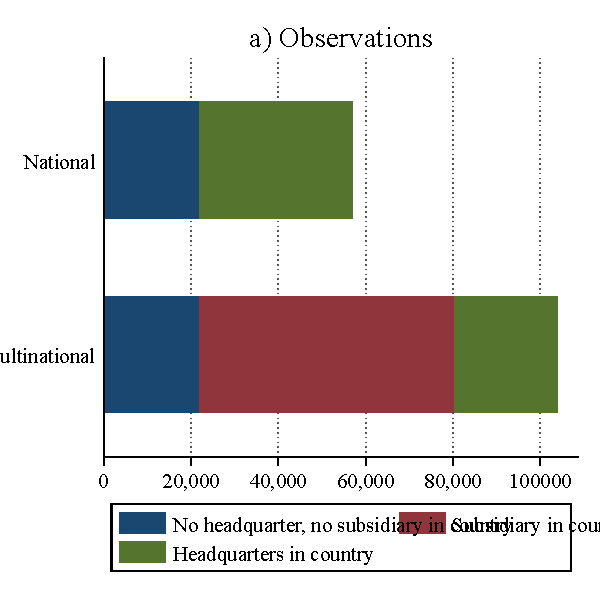
\includegraphics[width=.4\linewidth]{../output/figures/hq_sub_obs.pdf}
		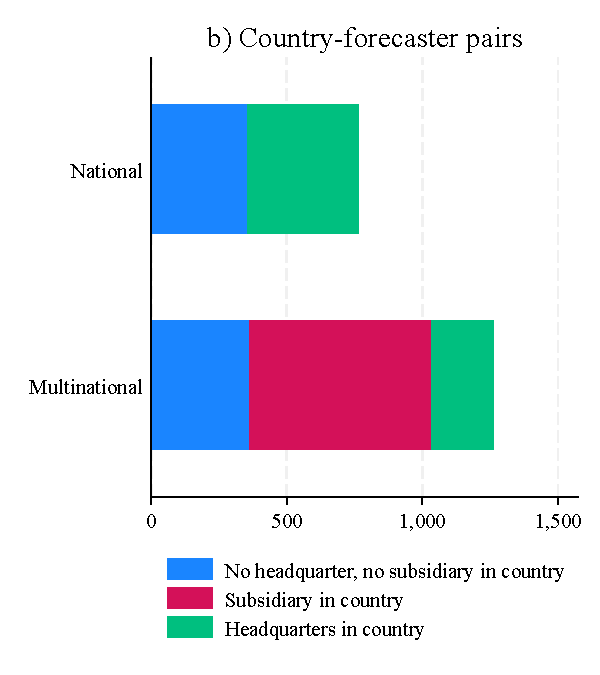
\includegraphics[width=.4\linewidth]{../output/figures/hq_sub_pairs.pdf}
\end{center}
	\caption{Distribution of forecasts and country-forecaster pairs conditional on Location and Scope of Forecaster}
	\label{fig:hq_sub_obs}
	\begin{fignote}
		\textit{Notes:} The figure shows the distribution of the forecasts and country-forecaster pairs conditional on the location and scope of the forecaster. A forecast is either provided by a forecaster with headquarters located in the country, or by a forecaster with no headquarters but with at least a subsidiary located in the country, or by a forecaster with neither headquarters or subsidiaries located in the country. Multinational forecasters have subsidiaries in countries other than the one where their headquarters are located. National forecasters have only subsidiaries in the same country as their headquarters.
	\end{fignote}
\end{figure}

\begin{figure}[H]
\begin{center}
		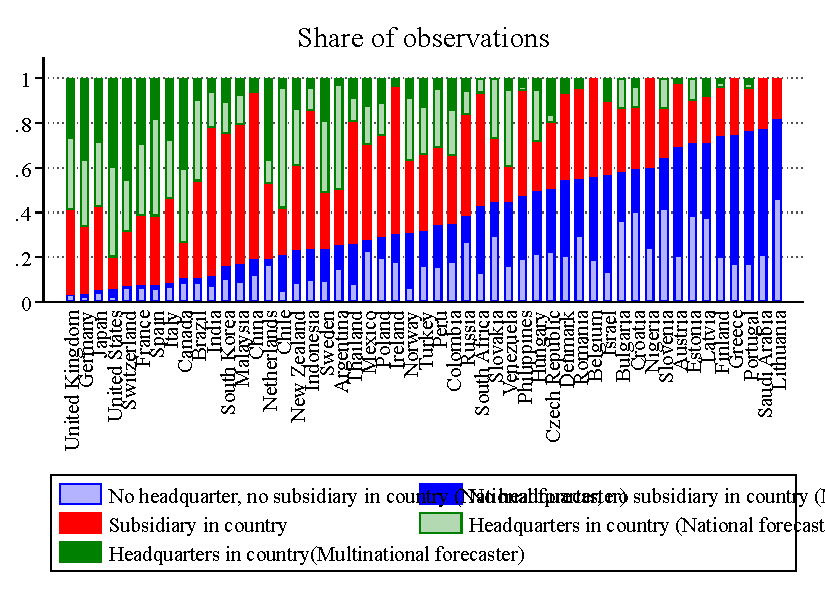
\includegraphics[width=.9\linewidth]{../output/figures/hq_sub_obs_by_cty.pdf}
\end{center}
	\caption{Proportion of forecasts conditional on Location and Scope of Forecaster, by country}
	\label{fig:hq_sub_obs_by_cty}
	\begin{fignote}
		\textit{Notes:} The figure shows the distribution of the forecasts conditional on the location and scope of the forecaster. A forecast is either provided by a forecaster with headquarters located in the country, or by a forecaster with no headquarters but with at least a subsidiary located in the country, or by a forecaster with neither headquarters or subsidiaries located in the country. Multinational forecasters have subsidiaries in countries other than the one where their headquarters are located. National forecasters have only subsidiaries in the same country as their headquarters.
	\end{fignote}
\end{figure}

\begin{figure}[H]
\begin{center}
		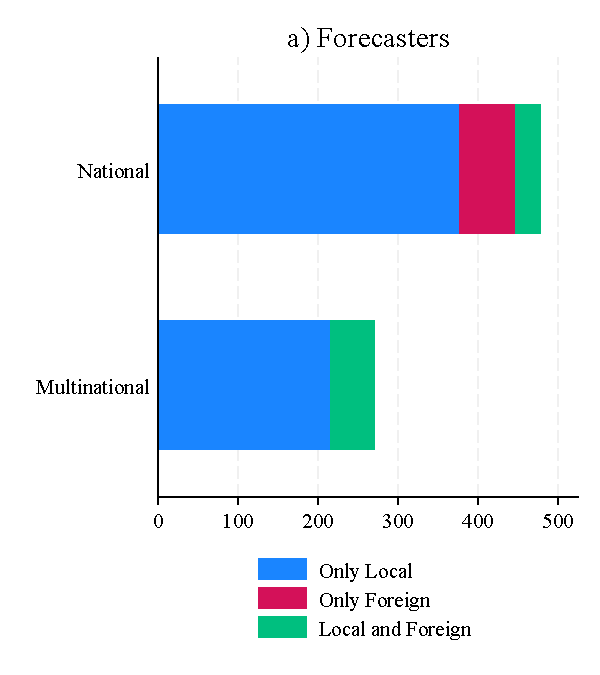
\includegraphics[width=.4\linewidth]{../output/figures/loc_for_inst.pdf}
		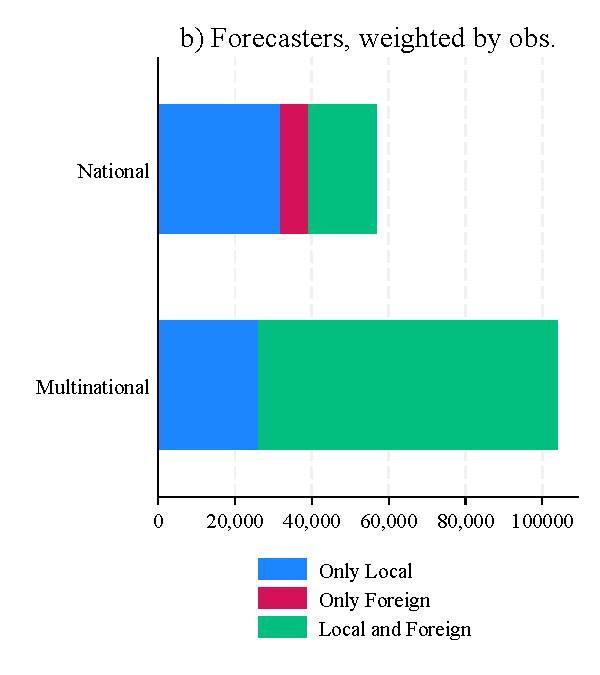
\includegraphics[width=.4\linewidth]{../output/figures/loc_for_obs.pdf}	
	\caption{Forecasters publishing Local and Foreign Forecasts}
		\label{fig:loc_for}
\end{center}

	\begin{fignote}
		\textit{Notes:} The figure shows the distribution of the forecasters depending on the nature of their forecasts. A forecaster either provides local forecasts only, or foreign forecasts only, or both local and foreign forecasts.
	\end{fignote}
\end{figure}

\begin{figure}[h]
\begin{center}
		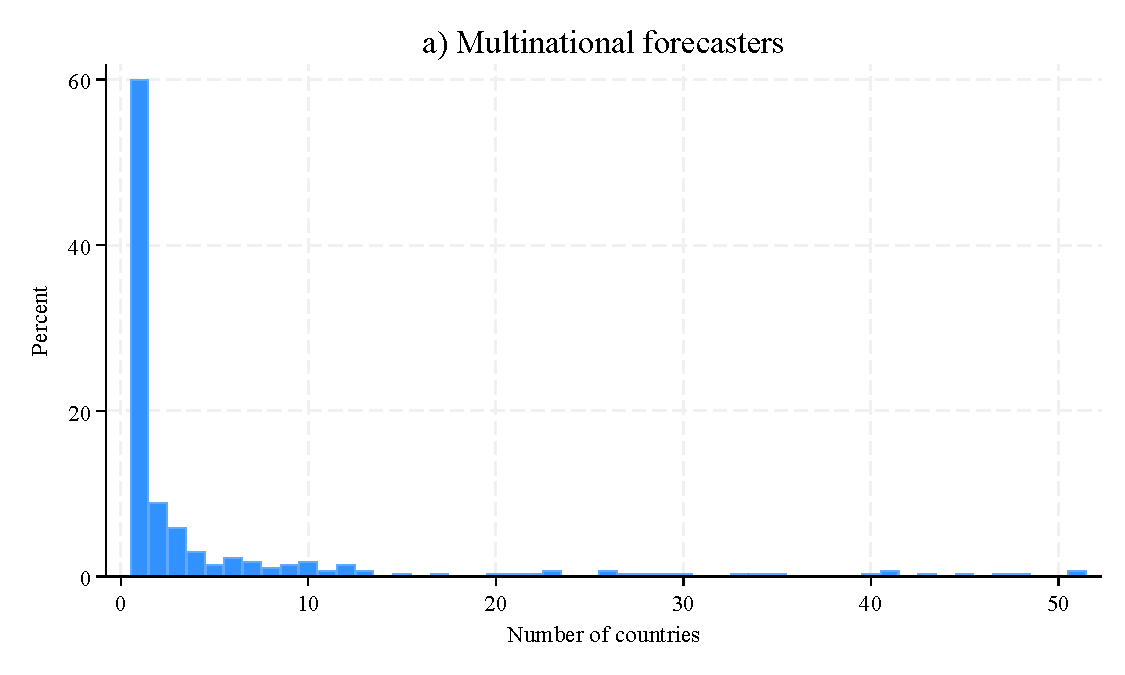
\includegraphics[width=.4\linewidth]{../output/figures/hist_mult.pdf}
		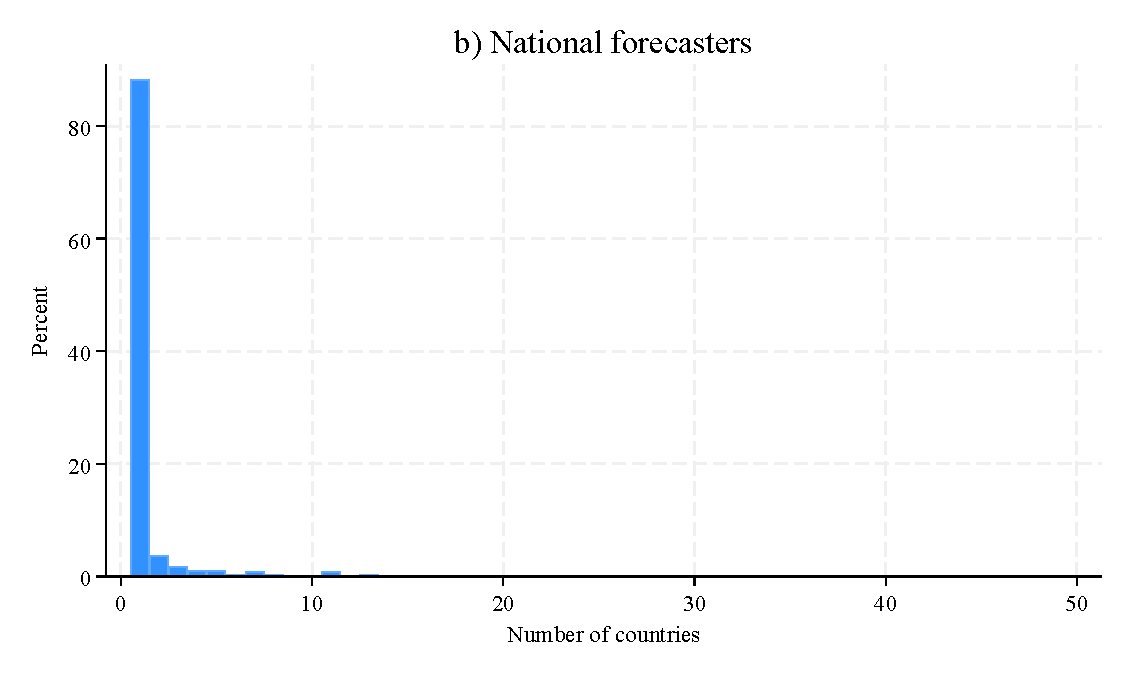
\includegraphics[width=.4\linewidth]{../output/figures/hist_nat.pdf}	
	\caption{Number of countries in forecasters' portfolio}
	\label{fig:hist}
\end{center}
	\begin{fignote}
		\textit{Notes:} The figure shows the distribution, across forecasters, of the number of countries that are in a forecaster's portfolio, depending of the forecaster's scope (multinational or national firm). A country is in a forecaster's portfolio if the forecaster provides forecasts for that country.
	\end{fignote}
\end{figure}

%%%% ERRORS
\newpage



\begin{figure}[h]
	
		\begin{subfigure}[b]{0.48\textwidth}
		\centering
		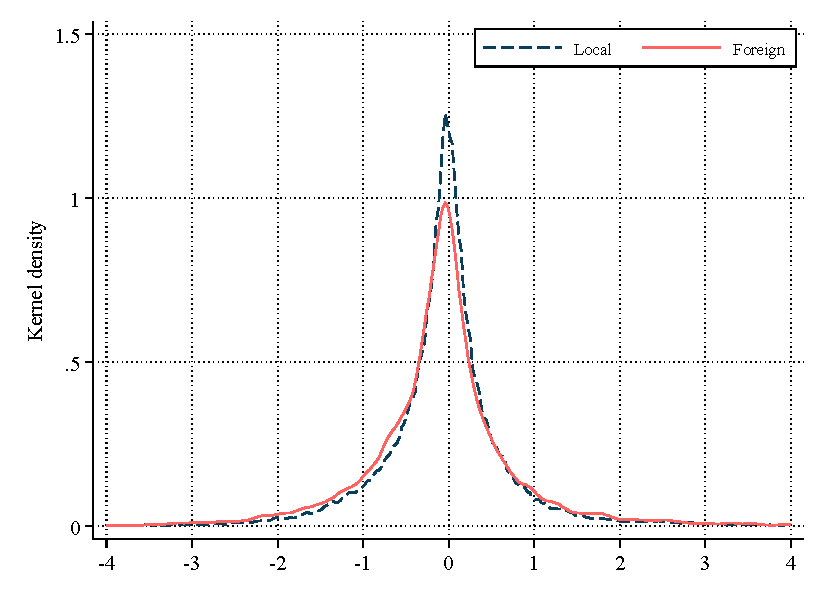
\includegraphics[width=1\linewidth]{../output/figures/cpi_current_FE_density}
		\caption{$Error_{ijt,t}^m$: $\text{CPI}_t$ }
		\label{fig:error_density_cpi_c}
	\end{subfigure}
	\hfill
	\begin{subfigure}[b]{0.48\textwidth}
		\centering
		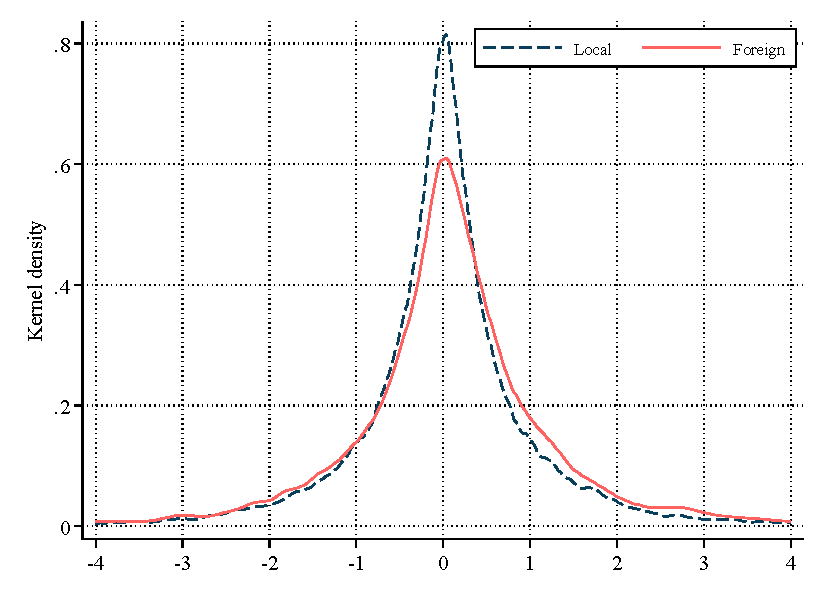
\includegraphics[width=1\linewidth]{../output/figures/gdp_current_FE_density}
		\caption{$Error_{ijt,t}^m$. $\text{GDP}_t$ }
		\label{fig:error_density_gdp_c}
	\end{subfigure}
	
		\begin{subfigure}[b]{0.48\textwidth}
		\centering
		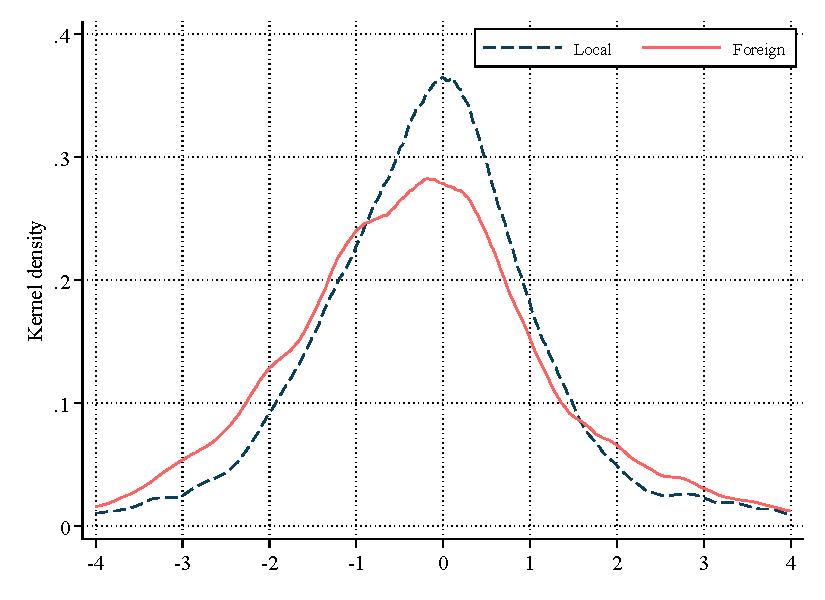
\includegraphics[width=1\linewidth]{../output/figures/cpi_future_FE_density}
		\caption{$Error_{ijt,t}^m$: $\text{CPI}_{t+1}$ }
		\label{fig:error_density_cpi_f}
	\end{subfigure}
	\hfill
	\begin{subfigure}[b]{0.48\textwidth}
		\centering
		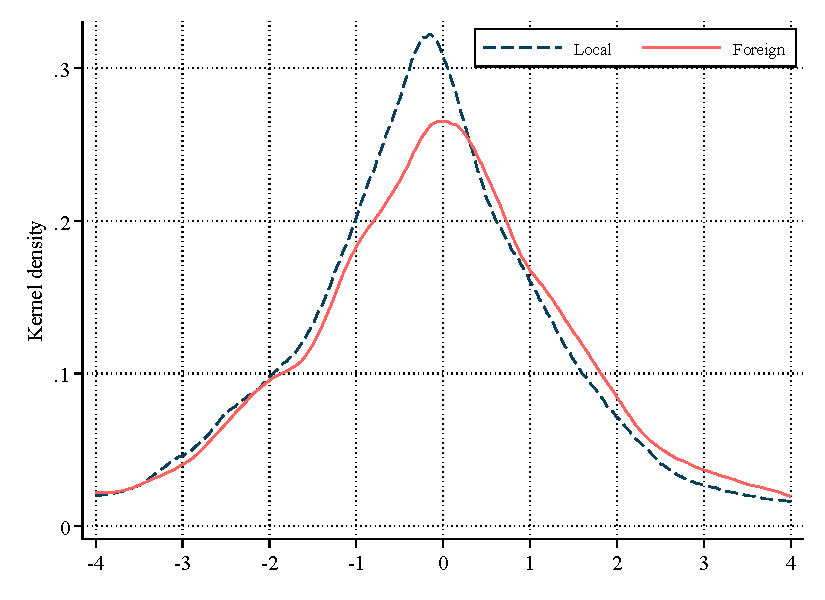
\includegraphics[width=1\linewidth]{../output/figures/gdp_future_FE_density}
		\caption{$Error_{ijt,t}^m$. $\text{GDP}_{t+1}$ }
		\label{fig:error_density_gdp_f}
	\end{subfigure}
	
	\caption{Distribution of errors}
	\label{fig:errors}
	\begin{fignote}
		\textit{Notes:} Panels (a) and (b) display the density of the current year forecast error $Error_{ijt,t}^m$ conditional on the location of the forecaster. Panels (c) and (d) display the density of the future year forecast error $Error_{ijt,t+1}^m$ conditional on the location of the forecaster. The population corresponds to all the country-forecaster-year units.
	\end{fignote}
\end{figure}




\begin{figure}[H]
	
		\begin{subfigure}[b]{0.48\textwidth}
		\centering
		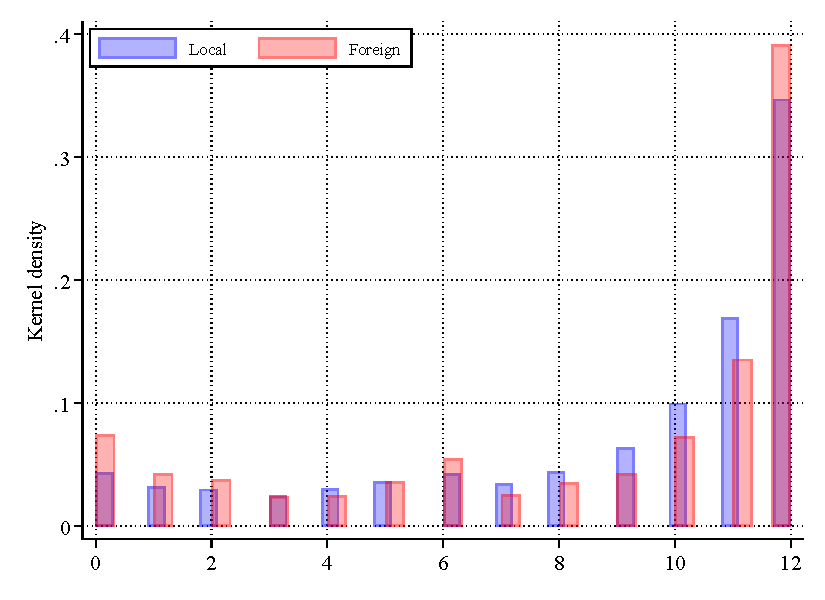
\includegraphics[width=1\linewidth]{../output/figures/cpi_current_N_density}
		\caption{$N_{ijt}$: $\text{CPI}_t$ }
		\label{fig:cpi_current_N_density}
	\end{subfigure}
	\hfill
	\begin{subfigure}[b]{0.48\textwidth}
		\centering
		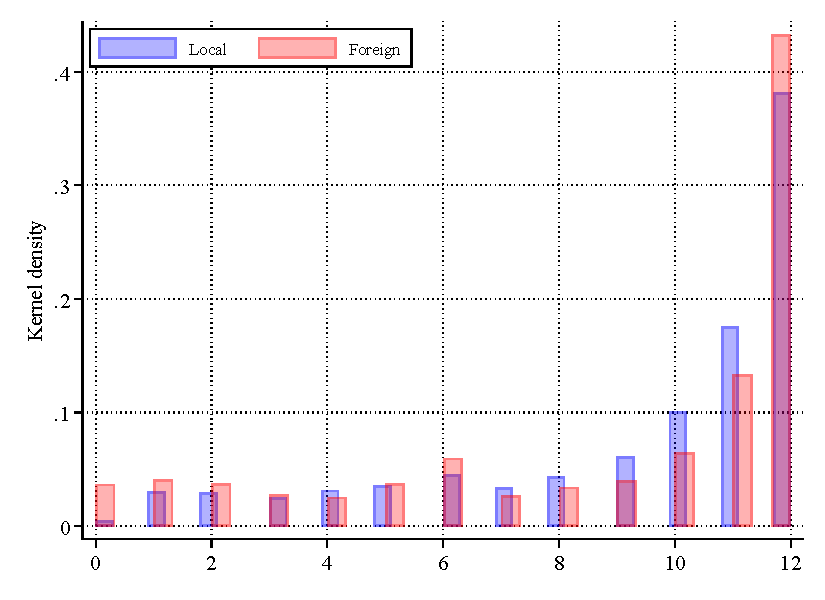
\includegraphics[width=1\linewidth]{../output/figures/gdp_current_N_density}
		\caption{$N_{ijt}$: $\text{GDP}_t$}
		\label{fig:gdp_current_N_density}
		\end{subfigure}
	
	\begin{subfigure}[b]{0.48\textwidth}
		\centering
		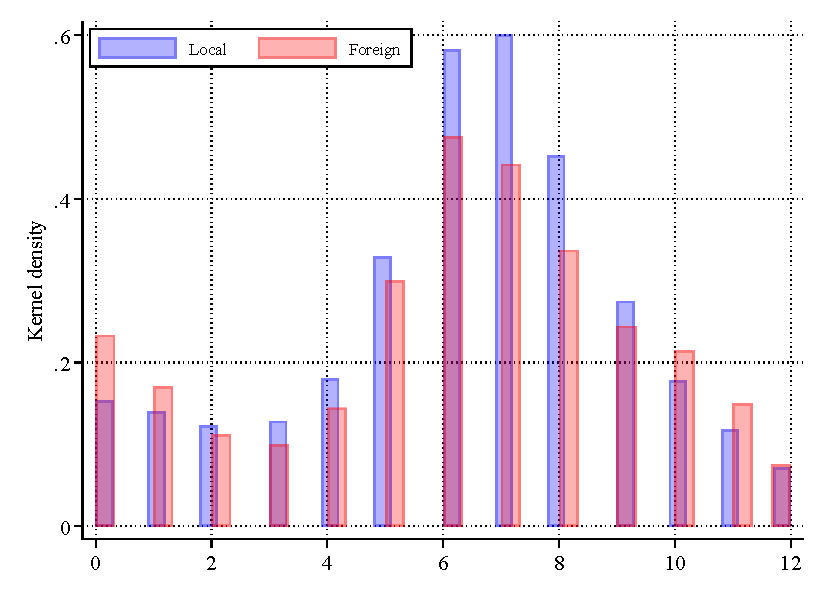
\includegraphics[width=1\linewidth]{../output/figures/cpi_current_N_density2}
		\caption{$N_{ijt}$: $\text{CPI}_{t}$ }
		\label{fig:cpi_current_N_density2}
	\end{subfigure}
	\hfill
	\begin{subfigure}[b]{0.48\textwidth}
		\centering
		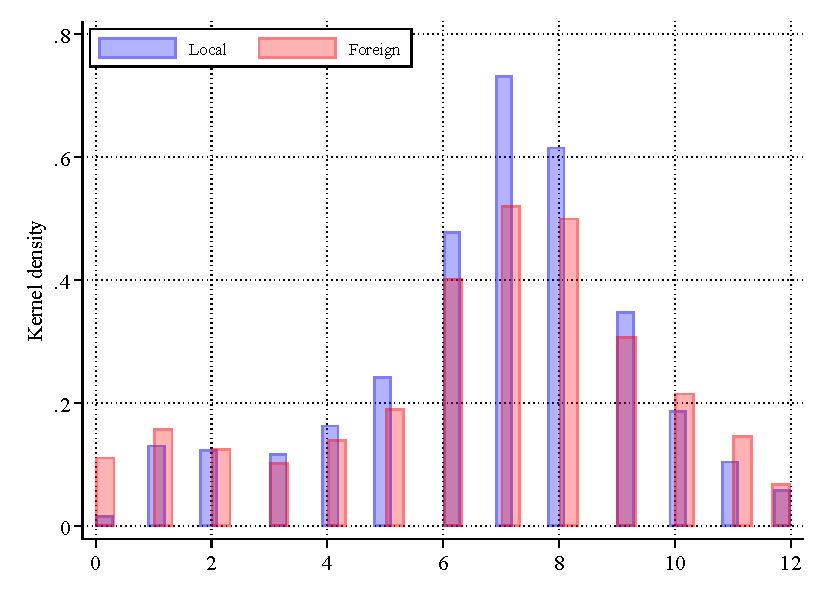
\includegraphics[width=1\linewidth]{../output/figures/gdp_current_N_density2}
		\caption{$N_{ijt}$: $\text{GDP}_{t}$}
		\label{fig:gdp_current_N_density2}
	\end{subfigure}
	
	\caption{Distribution of the number of yearly updates}
	\label{fig:updates}
	\begin{fignote}
		\textit{Notes:} Panels (a) and (b) display the histograms of the number of current year forecasts $N_{ijt}$ by location, where we consider all the published forecast. Panels (c) and (d) display the histograms of the number of current year forecasts by location, where we consider only the published forecasts that are distinct from the last published one.
	\end{fignote}
\end{figure}


%%%%%%% BIASES

\newpage
%\begin{figure}[H]
	%
	%\begin{subfigure}[b]{0.48\textwidth}
		%\centering
		%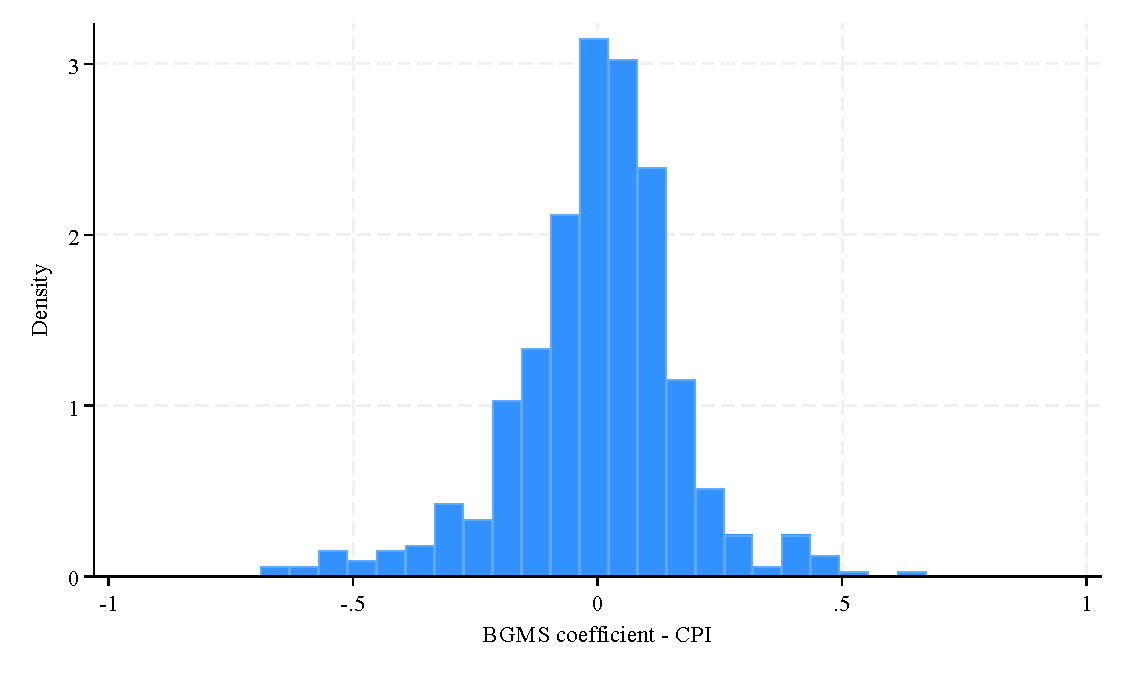
\includegraphics[width=1\linewidth]{Figures/dist_beta_cpi}
		%\caption{$\text{CPI}_t$ }
		%\label{fig:dist_beta_cpi}
	%\end{subfigure}
	%\hfill
	%\begin{subfigure}[b]{0.48\textwidth}
		%\centering
		%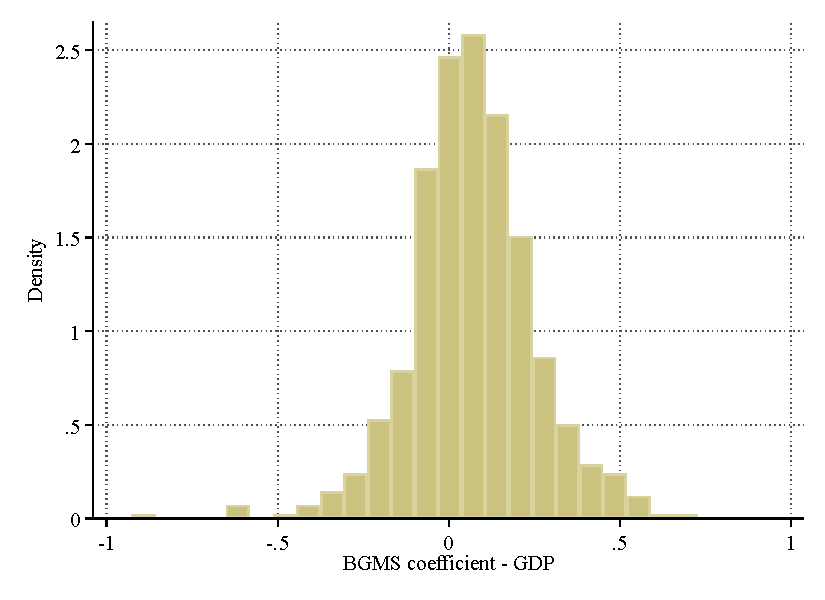
\includegraphics[width=1\linewidth]{Figures/dist_beta_gdp}
		%\caption{$\text{GDP}_t$ }
		%\label{fig:dist_beta_gdp}
	%\end{subfigure}
	%\caption{Distribution of $\beta^{BGMS}$ coefficients}
	%\label{app:fig:dist_beta}
	%\begin{fignote}
		%\textit{Notes:} The figure displays the distribution of the $\beta^{BGMS}$ coefficients estimated for each country-forecaster pair.
	%\end{fignote}
%\end{figure}

\begin{figure}[H]
	
	\begin{subfigure}[b]{0.48\textwidth}
		\centering
		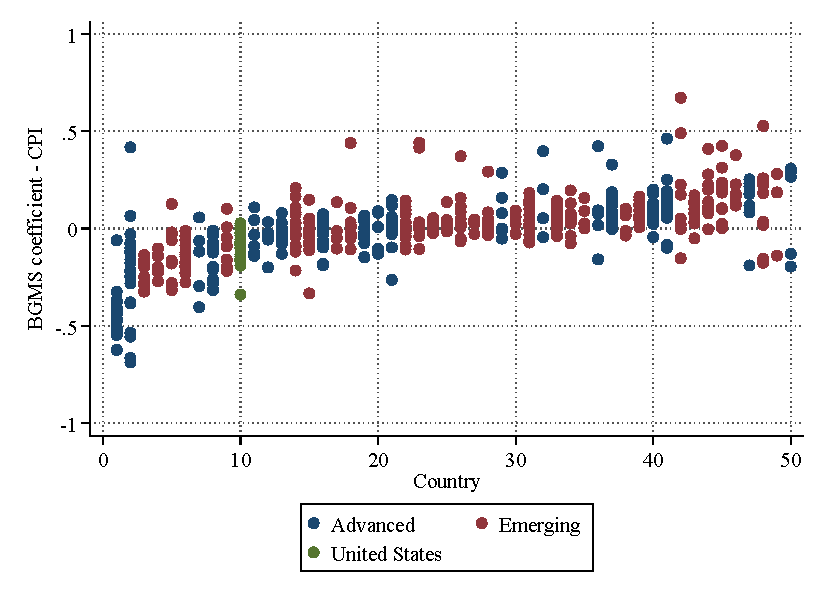
\includegraphics[width=1\linewidth]{../output/figures/dist_beta_cpi_cty}
		\caption{$\text{CPI}_t$ }
		\label{fig:dist_beta_cpi_cty}
	\end{subfigure}
	\hfill
	\begin{subfigure}[b]{0.48\textwidth}
		\centering
		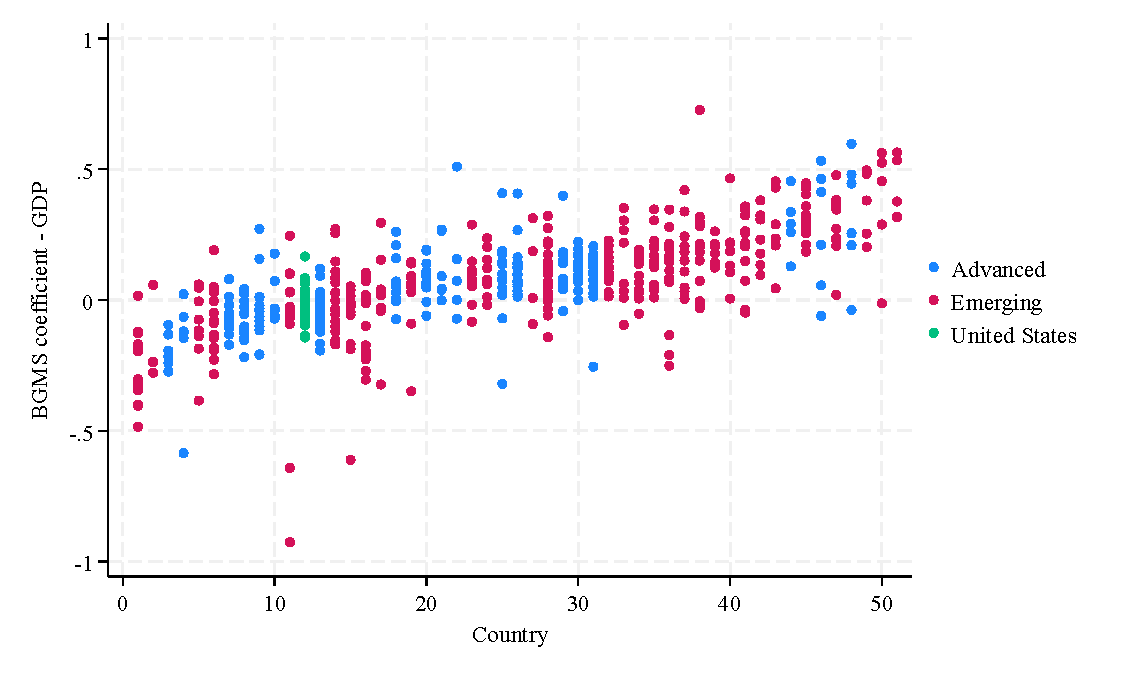
\includegraphics[width=1\linewidth]{../output/figures/dist_beta_gdp_cty}
		\caption{$\text{GDP}_t$ }
		\label{fig:dist_beta_gdp_cty}
	\end{subfigure}
	\caption{$\beta^{BGMS}$ coefficients by country}
	\label{app:fig:dist_beta_cty}
	\begin{fignote}
		\textit{Notes:} The figure displays the $\beta^{BGMS}$ coefficients estimated for each country-forecaster pair, by country, where countries are ranked by their median value.
	\end{fignote}
\end{figure}

\begin{landscape}
\begin{figure}[H]
	
	\begin{subfigure}[b]{0.65\textwidth}
		\centering
		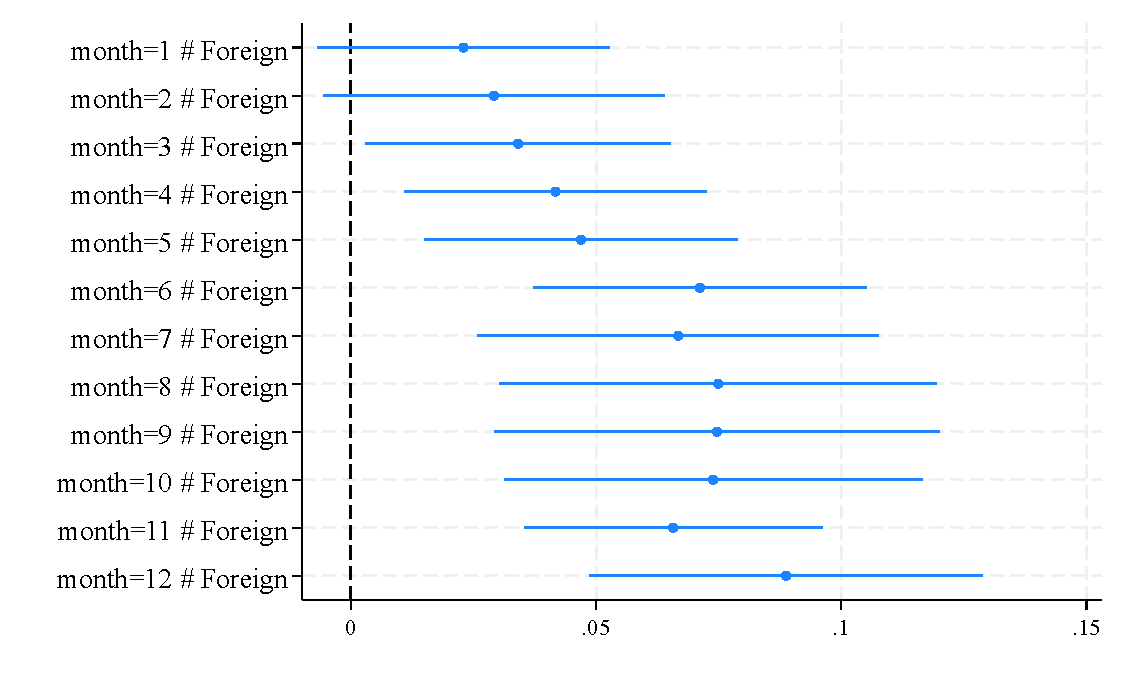
\includegraphics[width=1\linewidth]{../output/figures/heterogeneity_by_month.pdf}
		\caption{Foreign penalty by month}
	\end{subfigure}
	\hfill
	\begin{subfigure}[b]{0.65\textwidth}
		\centering
		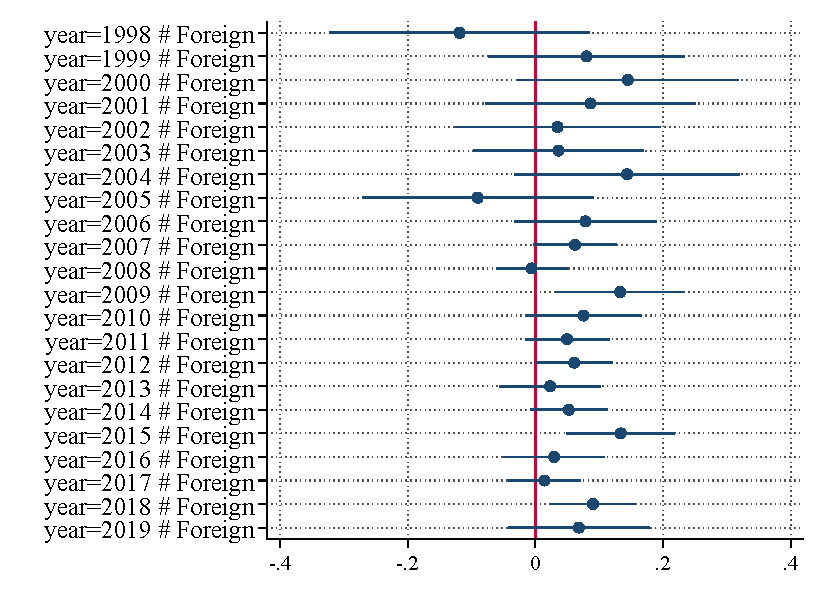
\includegraphics[width=1\linewidth]{../output/figures/heterogeneity_by_year.pdf}
		\caption{Foreign penalty by year}
	\end{subfigure}
	\hfill
	\begin{subfigure}[b]{0.65\textwidth}
		\centering
		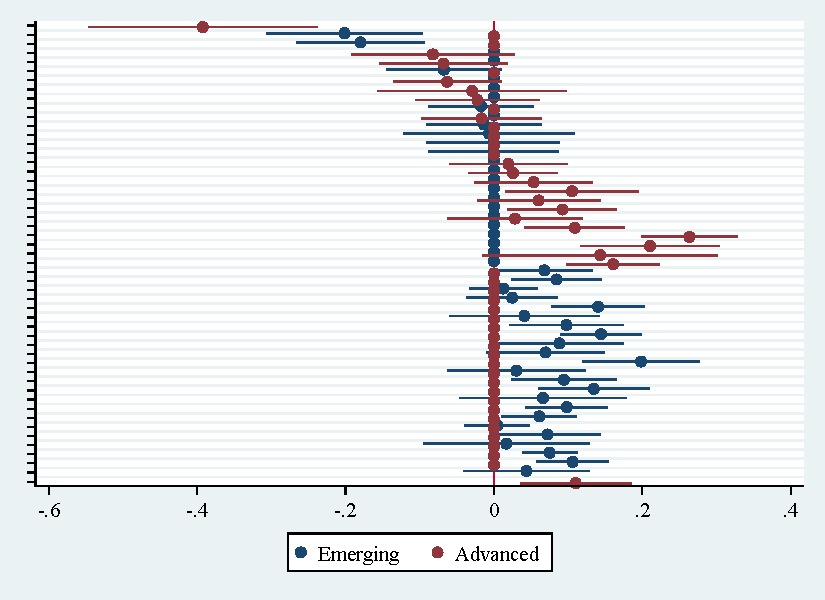
\includegraphics[width=1\linewidth]{../output/figures/heterogeneity_by_cty.pdf}
		\caption{Foreign penalty by country}
	\end{subfigure}
	\hfill
	\begin{subfigure}[b]{0.65\textwidth}
		\centering
		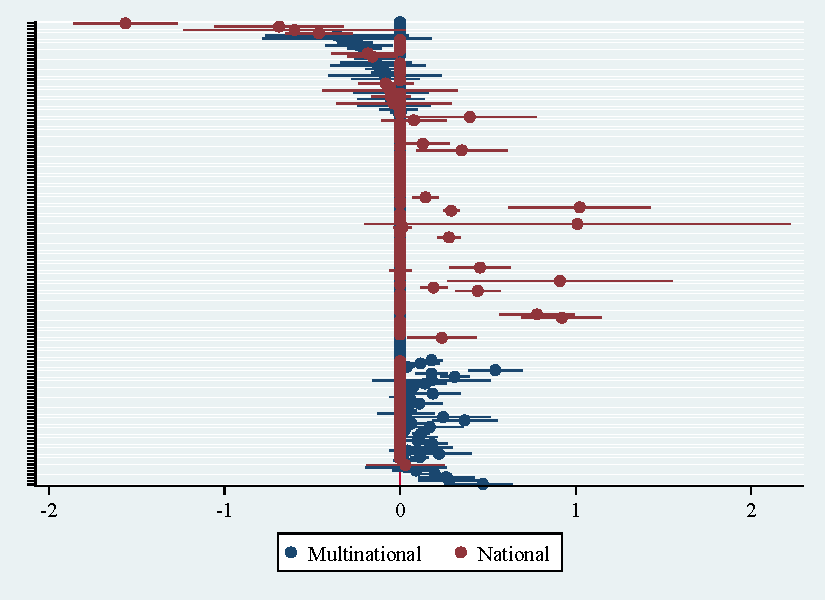
\includegraphics[width=1\linewidth]{../output/figures/heterogeneity_by_for.pdf}
		\caption{Foreign penalty by forecaster}
	\end{subfigure}
		\caption{Heterogeneity in Foreign penalty}
	\begin{fignote}
		\textit{Notes:} The figure displays the Foreign coefficients per year, month, country and forecaster. These estimates are obtained by estimating Equation \eqref{eq:heterogeneity} with $X_{ijt,h}^{m,x}$ successively replaced with the categorical variables year, month, and country and forecaster.
	\end{fignote}
	\label{fig:heterogeneity}
\end{figure}
\end{landscape}

%%%%%%%%%%%%%%%%%%%%%%%%%%%%%%%%%%%%%%%%%%%%%%%%%%%%%%%%%%
\newpage
\section{Proofs}
%%%%%%%%%%%%%%%%%%%%%%%%%%%%%%%%%%%%%%%%%%%%%%%%%%%%%%%%%%%%%%%%%%%%%%%%%%%%%%%%%%%%%%%%%%%%
\subsection{Proof of Proposition \ref{prop:variance}}
\label{proof:variance}

We first demonstrate the following Lemma:

\begin{lemma}\label{lemma:variance} Under Assumption \ref{ass:nobias} (no behavioral biases), the variance of errors is given by:
\begin{equation}\begin{array}{lll}V(Error_{ijt,t-1}^m)&=V[x_{jt}-E_{ijt-1}^m(x_{jt})]&=\frac{\gamma^{-1}}{1-\rho_{j}^2(1-G_{ij}^m)}\\
																 V(Error_{ijt,t}^m)&=V[x_{jt}-E_{ijt}^m(x_{jt})]&=\frac{\gamma^{-1}(1-G_{ij}^m)}{1-\rho_{j}^2(1-G_{ij}^m)}
																\end{array}\label{eq:variance}\end{equation}
Both variances are decreasing in $G_{jk}^m$.
\end{lemma}

\begin{proof}

Under Assumption \ref{ass:nobias}, we have $\hat\rho_{ij}=\rho_j$ and $\hat\tau_{ij}^m=\tau_{ij}^m$.

The model can be written as follows:
\begin{equation}\begin{array}{ll}x_{jt}	&=\rho_jx_{jt-1}+\epsilon_{jt}\\
								s_{ijt}^m&=x_{jt}+v_{ijt}^m\\
								\end{array}\label{eq:model}\end{equation}
with $v_{ijt}^m=h_{ij}^m(\kappa^m_{j})^{-1/2}u_{jt}^m+(1-h_{ij}^m)(\tau^m_{ij})^{-1/2}e^m_{ijt}$, $v_{ijt}^m\sim\textsl{N}(0,(\kappa_j^m+\tau_{ij}^m)^{-1/2})$. We denote $\lambda_{ij}^m=\kappa_j^m+\tau_{ij}^m$.

Denote the one step-ahead forecast error associated to the Kalman filter by $\Phi_{ij}^m=V(Error_{ijt,t-1}^m)=V[x_{jt}-E_{ijt-1}^m(x_{jt})]$. We can find $\Phi_{ij}^m$ from the Riccati equation $$\Phi_{ij}^m=\rho_j^2[\Phi_{ij}^m-\Phi_{ij}^m(\Phi_{ij}^m+(\lambda_{ij}^m)^{-1})^{-1}\Phi_{ij}^m]+\gamma_j^{-1}.$$ Denote the gain of the Kalman filter by $$G_{ij}^m=\Phi_{ij}^m(\Phi_{ij}^m+(\lambda_{ij}^m)^{-1})^{-1}.$$ Substituting in the Riccati equation, we obtain
$$\Phi_{ij}^m=\rho_j^2(1-G_{ij}^m)\Phi_{ij}^m+\gamma_j^{-1},$$
hence the first result of the Lemma.

Now denote the forecast error in the Kalman filter with $\Omega_{ij}^m=V(Error_{ijt,t}^m)=V[x_{jt}-E_{ijt}^m(x_{jt})]$
We can use recursions of the Kalman filter to relate $\Omega_{ij}^m$ and $\Phi_{ij}^m$:
$$\Omega_{ij}^m=\Phi_{ij}^m-G_{ij}^m(\Phi_{ij}^m+(\lambda_{ij}^m)^{-1})G_{ij}^{m'}$$
Replacing $G_{jk}^{m'}$, we obtain
$$\begin{array}{ll}\Omega_{ij}^m&=\Phi_{ij}^m-G_{ij}^m(\Phi_{ij}^m+(\lambda_{ij}^m)^{-1})[\Phi_{ij}^m(\Phi_{ij}^m+(\lambda_{ij}^m)^{-1})^{-1}]'\\
															&=\Phi_{ij}^m-G_{ij}^m\Phi_{ij}^m\\
															&=(1-G_{ij}^m)\Phi_{ij}^m\\
															\end{array}$$
Hence the second result of the Lemma.
\end{proof}

Since $G_{ij}^m$ is increasing in $\tau_{ij}^m$, then the variances are decreasing in $\tau_{ij}^m$. This proves Proposition \ref{prop:variance}.

Note that solving the Riccati equation gives us an expression for $\Phi_{ij}^m$:
\begin{equation}\Phi_{ij}^m=\frac{1}{2}\left(\gamma_j^{-1}-(1-\rho_j^2)(\lambda_{ij}^m)^{-1}+\sqrt{(\gamma_j^{-1}-(1-\rho_j^2)(\lambda_{ij}^m)^{-1})^2+4\gamma_j^{-1}(\lambda_{ij}^m)^{-1}}\right)\label{eq:Phi}\end{equation}
and for $G_{ij}$:
$$G_{ij}^m=1-\frac{2}{\lambda_{ij}^m/\gamma_j+1+\rho_j^2+\sqrt{(\lambda_{ij}^m/\gamma_j-(1-\rho_j^2))^2+4\lambda_{ij}^m/\gamma_j}}$$
which is an increasing function of $\lambda_{ij}^m$ and hence of $\tau_{ij}^m$.


%%%%%%%%%%%%%%%%%%%%%%%%%%%%%%%%%%%%%%%%%%%%%%%%%%%%%%%%%%%%%%%%%%%%%%%%%%%%%%%%%%%%%%%%%%%%
\subsection{Proof of Proposition \ref{prop:BGMS}}
\label{proof:BGMS}

First, we demonstrate the following Lemma:
\begin{lemma}\label{lemma:BGMS} Estimating Equation \eqref{eq:BGMS} for each $i=1,..N$, $j=1,..J$ and $m=1,..12$ by OLS gives the following coefficients:
$$\beta^{BGMSm}_{ij}=-(\hat\rho_{ij}-\rho_j)\beta_{1ij}^m - [(\tau_{ij}^m)^{-1}-(\hat\tau_{ij}^m)^{-1}]\beta_{2ij}^m$$
$\beta_{1ij}^m$ and $\beta_{2ij}^m$ are described below. They depend on the country-invariant parameters $\kappa_j^m$ and $\rho_j$ but also on the forecaster-specific beliefs $\hat\tau_{ij}^m$ and $\hat\rho_{ij}$.
\end{lemma}
A negative coefficient reflects an over-reaction of forecasters to their information. This over-reaction can arise from over-confidence ($\hat\tau_{ij}^m-\tau_{ij}^m>0$) or from over-extrapolation ($\hat\rho_{ij} -\rho_j>0$).

\begin{proof}

Notice that $E_{ijt}^m(x_{jt})$ can be rewritten in its moving-average form as follows:
\begin{equation}E_{ijt}^m(x_{jt})=\frac{G_{ij}^m}{1-(1-G_{ij}^m)\hat\rho_{ij}L}s_{ijt}^m\label{eq:ma}\end{equation}
Forecast revision can then be written as
\begin{equation}\begin{array}{ll}Revision_{ijt}^m&=E_{ijt}^m(x_{jt})-E_{ijt-1}^m(x_{jt})\\
																								&=E_{ijt}^m(x_{jt})-\hat\rho_{ij}E_{ijt-1}^m(x_{jt-1})\\
																								&=\frac{G_{ij}^m[1-\hat\rho_{ij}L]}{1-(1-G_{ij}^m)\hat\rho_{ij}L}s_{ijt}^m\\
																								&=\frac{G_{ij}^m[1-\hat\rho_{ij}L]}{1-(1-G_{ij}^m)\hat\rho_{ij}L}(x_{jt}+v_{ijt}^m)\\
																								\end{array}\label{eq:revision2}\end{equation}
and the error as
\begin{equation}\begin{array}{ll}Error_{ijt,t}^m&=x_{jt}-E_{ijt}^m(x_{jt})\\
																							&=x_{jt}-\frac{G_{ij}^m}{1-(1-G_{ij}^m)\hat\rho_{ij}L}s_{ijt}^m\\
																							&=\left(1-\frac{G_{ij}^m}{1-(1-G_{ij}^m)\rho_{ij}L}\right)x_{jt}-\frac{G_{ij}^m}{1-(1-G_{ij}^m)\hat\rho_{ij}L}v_{ijt}^m\\
																								\end{array}\label{eq:error2}\end{equation}
with $v_{ijt}^m=h_{ij}^m(\kappa_j^m)^{-1/2}u_{jt}^m+(1-h_{ij}^m)(\tau_{ij}^m)^{-1/2}e_{ijt}^m$ is the total noise.


The estimated OLS coefficient $\beta^{BGMSm}_{ij}$ is given by
$$\beta^{BGMSm}_{ij}  = \frac{Cov\left(Error_{ijt}^m,Revision_{ijt}^m\right)}{V\left(Revision_{ijt}^m\right)}$$
We define $\tilde Error_{ijt,t}^m$ as the error if the persistence and private signal precisions were the ones corresponding to the forecaster's beliefs:
\begin{equation}\tilde Error_{ijt,t}^m=\left(1-\frac{G_{ij}^m}{1-(1-G_{ij}^m)   \hat\rho_{ij}   L}\right)\tilde x_{ijt}-\frac{G_{ij}^m}{1-(1-G_{ij}^m)\hat\rho_{ij}L}\tilde v_{ijt}^m\label{eq:tildeerror}\end{equation}
with $\tilde x_{ijt}=\epsilon_{jt}/(1-\hat\rho_{ij}L)$ and $\tilde v_{ijt}^m=h_{ij}^m(\kappa_j^m)^{-1/2}u_{jt}^m+(1-h_{ij}^m)(\hat\tau_{ij}^m)^{-1/2}e_{ijt}^m$. We define $\tilde Revision_{ijt,t}^m$ similarly:
$$\tilde Revision_{ijt}^m=\frac{G_{ij}^m[1-\hat\rho_{ij}L]}{1-(1-G_{ij}^m)\hat\rho_{ij}L}(\tilde x_{ijt}+\tilde v_{ijt}^m)$$

We then use the fact that the forecaster's expectations are rational conditional on their beliefs: $Cov(\tilde Error_{ijt,t}^m,\tilde Revision_{ijt}^m)=0$ to determine the covariance of the actual errors and revisions:
$$\begin{array}{rl}Cov\left(Error_{ijt}^m,Revision_{ijt}^m\right)=& Cov\left(Error_{ijt}^m-\tilde Error_{ijt}^m,\tilde Revision_{ijt}^m\right) \\
&+ Cov\left(\tilde Error_{ijt}^m,Revision_{ijt}^m-\tilde Revision_{ijt}^m\right)\\
&+Cov\left(Error_{ijt}^m-\tilde Error_{ijt}^m,Revision_{ijt}^m-\tilde Revision_{ijt}^m\right)\\
=&Cov\left(\left(1-\frac{G_{ij}^m}{1-(1-G_{ij}^m)\hat\rho_{ij}L}\right)(x_{jt}-\tilde x_{ijt}),\frac{G_{ij}^m(1-\hat\rho_{ij}L)}{1-(1-G_{ij}^m)\hat\rho_{ij}L}\tilde x_{ijt}\right)\\
&+Cov\left(\left(1-\frac{G_{ij}^m}{1-(1-G_{ij}^m)\hat\rho_{ij}L}\right)\tilde x_{ijt},\frac{G_{ij}^m(1-\hat\rho_{ij}L)}{1-(1-G_{ij}^m)\hat\rho_{ij}L}(x_{jt}-\tilde x_{ijt})\right)\\
&+Cov\left(\left(1-\frac{G_{ij}^m}{1-(1-G_{ij}^m)\hat\rho_{ij}L}\right)(x_{jt}-\tilde x_{ijt}),\frac{G_{ij}^m(1-\hat\rho_{ij}L)}{1-(1-G_{ij}^m)\hat\rho_{ij}L}(x_{jt}-\tilde x_{ijt})\right)\\
&-Cov\left(\frac{G_{ij}^m}{1-(1-G_{ij}^m)\hat\rho_{ij}L}\tilde v_{ijt}^m,\frac{G_{ij}^m(1-\hat\rho_{ij}L)}{1-(1-G_{ij}^m)\hat\rho_{ij}L}( v_{ijt}^m-\tilde v_{ijt}^m)\right)\\
&-Cov\left(\frac{G_{ij}^m}{1-(1-G_{ij}^m)\hat\rho_{ij}L}(v_{ijt}^m-\tilde v_{ijt}^m),\frac{G_{ij}^m(1-\hat\rho_{ij}L)}{1-(1-G_{ij}^m)\hat\rho_{ij}L}\tilde v_{ijt}^m\right)\\
&-Cov\left(\frac{G_{ij}^m}{1-(1-G_{ij}^m)\hat\rho_{ij}L}(v_{ijt}^m-\tilde v_{ijt}^m),\frac{G_{ij}^m(1-\hat\rho_{ij}L)}{1-(1-G_{ij}^m)\hat\rho_{ij}L}(v_{ijt}^m-\tilde v_{ijt}^m)\right)\\
=&-(\hat\rho_{ij}-\rho_j)G_{ij}^m(1-G_{ij}^m)\frac{2\hat\rho_{ij}(1-G_{ij}^m)(1-\rho_j^2)-(\hat\rho_{ij}-\rho_j)[1+\rho_j\hat\rho_{ij}(1-G_{ij}^m)]}{[1-\rho_j\hat\rho_{ij}(1-G_{ij}^m)][1-\rho_j^2][1-\hat\rho_{ij}^2(1-G_{ij}^m)^2]}\\
&-[(\tau_{ij}^m)^{-1}-(\hat\tau_{ij}^m)^{-1}]((1-h_{ij}^m) G_{ij}^m)^2\frac{1-\hat\rho_{ij}^2(1-G_{ij}^m)}{1-\hat\rho_{ij}^2(1-G_{ij}^m)^2}\\
\end{array}$$

We used
$$\begin{array}{ll}
\tilde Error_{ijt}^m&=(1-G_{ij}^m)\sum_{s=0}^{+\infty}(1-G_{ij}^m)^s\hat\rho_{ij}^sL^s\epsilon_{jt}\\
&-G_{ij}^m\sum_{s=0}^{+\infty}(1-G_{ij}^m)^s\hat\rho_{ij}^sL^s h_{ij}^m(\hat\tau_{ij}^m)^{-1/2}e_{ijt}^m\\
\tilde Revision_{ijt}^m&=G_{ij}^m\sum_{s=0}^{+\infty}(1-G_{ij}^m)^s\hat\rho_{ij}^sL^s\epsilon_{jt}\\
&-G_{ij}^m\left(1-\frac{G_{ij}^m}{1-G_{ij}^m}\sum_{s=1}^{+\infty}(1-G_{ij}^m)^s\hat\rho_{ij}^sL^s \right) (1-h_{ij}^m)(\hat\tau_{ij}^m)^{-1/2}e_{ijt}^m\\
Error_{ijt}^m-\tilde Error_{ijt}^m&=\frac{-\left(\frac{\hat\rho_{ij}}{\rho_j}-1\right)(1-G_{ij}^m)}{1-(1-G_{ij}^m)\frac{\hat\rho_{ij}}{\rho_j}}\left(\sum_{s=0}^{+\infty}\rho_{ij}^sL^s-\sum_{s=0}^{+\infty}(1-G_{ij}^m)^s\hat\rho_{ij}^sL^s\right)\epsilon_{jt}\\
&-G_{ij}^m\sum_{s=0}^{+\infty}(1-G_{ij}^m)^s\hat\rho_{ij}^sL^s h_{ij}^m[(\tau_{ij}^m)^{-1/2}-(\hat\tau_{ij}^m)^{-1/2}]e_{ijt}^m\\
Revision_{ijt}^m-\tilde Revision_{ijt}^m&=\frac{-\left(\frac{\hat\rho_{ij}}{\rho_j}-1\right)G_{ij}^m}{1-(1-G_{ij}^m)\frac{\hat\rho_{ij}}{\rho_j}}\left(\sum_{s=0}^{+\infty}\rho_{ij}^sL^s-\sum_{s=0}^{+\infty}(1-G_{ij}^m)^s\hat\rho_{ij}^sL^s\right)\epsilon_{jt}\\
&-G_{ij}^m\left(1-\frac{G_{ij}^m}{1-G_{ij}^m}\sum_{s=1}^{+\infty}(1-G_{ij}^m)^s\hat\rho_{ij}^sL^s \right) (1-h_{ij}^m)[(\tau_{ij}^m)^{-1/2}-(\hat\tau_{ij}^m)^{-1/2}]e_{ijt}^m\\
\end{array}$$

We thus have
$$\beta_{1ij}^m =\frac{G_{ij}^m(1-G_{ij}^m)\frac{2\hat\rho_{ij}(1-G_{ij}^m)(1-\rho_j^2)-(\hat\rho_{ij}-\rho_j)[1+\rho_j\hat\rho_{ij}(1-G_{ij}^m)]}{[1-\rho_j\hat\rho_{ij}(1-G_{ij}^m)][1-\rho_j^2][1-\hat\rho_{ij}^2(1-G_{ij}^m)^2]}}{V\left(Revision_{ijt}^m\right)}$$
and
$$\beta_{2ij}^m =\frac{(h_{ij}^mG_{ij}^m)^2\frac{1-\hat\rho_{ij}^2(1-G_{ij}^m)}{1-\hat\rho_{ij}^2(1-G_{ij}^m)^2}}{V\left(Revision_{ijt}^m\right)}$$
with
$$\begin{array}{ll}V(Revision_{ijt}^m)=&\frac{(G_{ij}^m)^2}{1-\frac{\hat\rho_{ij}}{\rho_j}(1-G_{ij}^m)}\left(\frac{G_{ij}^m\frac{\hat\rho_{ij}}{\rho_j}[1-\hat\rho_{ij}^2(1-G_{ij})]}{[1-\rho_j\hat\rho_{ij}(1-G_{ij})][1-\hat\rho_{ij}^2(1-G_{ij})^2]}-(\hat\rho_{ij}-\rho_j)\frac{1-\rho_j\hat\rho_{ij}}{[1-\rho_j\hat\rho_{ij}(1-G_{ij})](1-\rho_j^2)}\right)\\
&+(G_{ij}^m)^2\left(1+\left(\frac{G_{ij}^m}{1-G_{ij}^m}\right)^2\frac{\hat\rho_{ij}^2(1-G_{ij}^m)^2}{1-\hat\rho_{ij}^2(1-G_{ij}^m)^2}\right)[(h_{ij}^m)^2\kappa_j^{-1}+(1-h_{ij}^m)^2\tau_{ij}^{-1}]\end{array}$$

Here we used
$$\begin{array}{ll}Revision_{ijt}^m=&\frac{G_{ij}^m}{1-\frac{\hat\rho_{ij}}{\rho_j}(1-G_{ij}^m)}\left(\frac{\hat\rho_{ij}}{\rho_j}\sum_{s=0}^{+\infty}(1-G_{ij}^m)^s\hat\rho_{ij}^sL^s-\left(\frac{\hat\rho_{ij}}{\rho_j}-1\right)\sum_{s=0}^{+\infty}\rho_{j}^sL^s\right)\epsilon_{jt}\\
&+G_{ij}^m\left(1-\frac{G_{ij}^m}{1-G_{ij}^m}\sum_{s=1}^{+\infty}(1-G_{ij}^m)^s\hat\rho_{ij}^sL^s\right)v_{ijt}^m\\
\end{array}$$

\end{proof}

According to Lemma \ref{lemma:BGMS}, while a non-zero coefficient can help detect the presence of behavioral biases, it suffers from one drawback in our context: the coefficient is a non-linear and potentially non-monotonic function of $\hat\tau_{ij}-\tau_{ij}$, $\hat\rho_{ij}-\rho_{j}$, the biases, but also of $\tau_{ij}$, the precision of private signals. Interpreting differences in coefficients is therefore not straightforward. To prove Proposition \ref{prop:BGMS}, we therefore linearize $\beta_{ij}^{BGMSm}$.

%We simply note here that $\beta_{1ij}^m$ and $\beta_{2ij}^m$, evaluated at $(\hat\tau_{ij}^m)^{-1}=(\tau_{ij}^m)^{-1}=(\tau_j^m)^{-1}$ and $\hat\rho_{ij}=\rho_j$, are both strictly positive, while $\hat\rho_{ij}-\rho_{j}$ and $(\tau_{ij}^m)^{-1}-(\hat\tau_{ij}^m)^{-1}$ are both equal to zero for $\hat\tau_{ij}^m=\tau_{ij}^m=\tau_j^m$ and $\hat\rho_{ij}=\rho_j$.

Note that $\beta_{1ij}^m$ and $\beta_{2ij}^m$ are functions of the parameters, so we denote $\beta_{1ij}^m=g_1\left((\hat\tau_{ij}^m)^{-1},(\tau_{ij}^m)^{-1},\hat\rho_{ij},\rho_j\right)$ and $\beta_{2ij}^m=g_2\left((\hat\tau_{ij}^m)^{-1},(\tau_{ij}^m)^{-1},\hat\rho_{ij},\rho_j\right)$. The first-order Taylor expansion for $\beta_{ij}^{BGMSm}$ around $(\hat\tau_{ij}^m)^{-1}=(\tau_{ij}^m)^{-1}=(\tau_j^m)^{-1}$ and $\hat\rho_{ij}=\rho_j$ is
$$\beta_{ij}^{BGMSm}\simeq -(\hat\rho_{ij}-\rho_j)g_1\left((\tau_{j}^m)^{-1},(\tau_{j}^m)^{-1},\rho_{j},\rho_j\right) - [(\tau_{ij}^m)^{-1}-(\hat\tau_{ij}^m)^{-1}]g_2\left((\tau_{j}^m)^{-1},(\tau_{j}^m)^{-1},\rho_{j},\rho_j\right)$$
We can show that $\hat\beta_{1j}^m=g_1\left((\tau_{j}^m)^{-1},(\tau_{j}^m)^{-1},\rho_{j},\rho_j\right)$ and $\hat\beta_{2j}^m=g_2\left((\tau_{j}^m)^{-1},(\tau_{j}^m)^{-1},\rho_{j},\rho_j\right)$ are both strictly positive, hence the result in Proposition \ref{prop:BGMS}.

%%%%%%%%%%%%%%%%%%%%%%%%%%%%%%%%%%%%%%%%%%%%%%%%%%%%%%%%%%%%%%%%%%%%%%%%%%%%%%%%%%%%%%%%%%%%
\subsection{Proof of Proposition \ref{prop:consensus}}
\label{proof:consensus}

First, we show the following Lemma:
\begin{lemma}\label{lemma:consensus} Suppose that Assumptions \ref{ass:nobias} and \ref{ass:loc_hom} are satisfied: there are no behavioral biases and the precision parameters are identical within foreign forecasters and within local forecasters. Estimating Equation \eqref{eq:consensus} for each $j=1,..J$, $m=1,..,12$ and $k=l,f$ by OLS gives the following coefficients:
$$\beta^{CGm}_{jk}=\frac{\frac{1-G_{jk}^m}{G_{jk}^m}\gamma^{-1}-[1-\rho_j^2(1-G_{jk}^m)]h_{jk}^2(\kappa_j^m)^{-1}}{\gamma^{-1}+[1-\rho_j^2(1-2G_{jk}^m)](h_{jk}^m)^2(\kappa_j^m)^{-1}}$$
\end{lemma}

\begin{proof}

Suppose that there are no behavioral biases (Assumption \ref{ass:nobias}): $\hat\rho_{ij}=\rho_j$ and $\hat\tau_{ij}^m=\tau_{ij}^m$, and that the precision parameters are identical within foreign forecasters and within local forecasters (Assumption \ref{ass:loc_hom}): $\tau_{ij}^m=\tau_{jl}^m$ if $i\in\mathcal{S}^l(j)$ and $\tau_{ij}^m=\tau_{jf}^m$ if $i\in\mathcal{S}^f(j)$, for all $j=1,..J$ and $m=1,..,12$.

The estimated OLS coefficient $\beta^{CGm}_{jk}$, for $k=l,f$, $m=1,..,12$ and $j=1,..,J$, is given by
\begin{equation}\begin{array}{ll}\beta^{CGm}_{jk}  = \frac{Cov\left(Error_{jkt}^m,Revision_{jkt}^m\right)}{V\left(Revision_{jkt}^m\right)}\label{eq:beta}\end{array}\end{equation}

And we can write:																
$$\begin{array}{ll}Cov\left(Error_{jkt}^m,Revision_{jkt}^m\right) &=Cov\left(\left(1-\frac{G_{jk}^m}{1-(1-G_{jk}^m)\rho_{j}L}\right)\frac{1}{1-\rho_{j}L}\epsilon_{jt},\frac{G_{jk}^m}{1-(1-G_{jk}^m)\rho_{j}L}\epsilon_{jt}\right)\\
&+Cov\left(-\frac{G_{jk}^m}{1-(1-G_{jk}^m)\rho_{j}L}h_{jk}^m(\kappa_j^m)^{-1/2}u_{jt}^m,\frac{G_{jk}^m[1-\rho_{j}L]}{1-(1-G_{jk}^m)\rho_{j}L}h_{jk}^m(\kappa_j^m)^{-1/2}u_{jt}^m\right)\\
&=\frac{G_{jk}^m(1-G_{jk}^m)}{1-\rho_{j}^2(1-G_{jk}^m)^2}\gamma^{-1} -(G_{jk}^m)^2\left(1-\frac{G_{jk}^m}{1-G_{jk}^m}\frac{\rho_{j}^{2}(1-G_{jk}^m)^{2}}{1-\rho_{j}^{2}(1-G_{jk}^m)^{2}}\right)(h_{jk}^m)^2(\kappa_j^m)^{-1}\\
\end{array}$$
and
$$\begin{array}{ll}V(Revision_{jkt}^m)&=(G_{jk}^m)^2\frac{1}{1-\hat\rho_{jk}^2(1-G_{jk}^m)^2}\gamma^{-1} + (G_{jk}^m)^2\left(1+\left(\frac{G_{jk}^m}{1-G_{jk}^m}\right)^2\frac{\hat\rho_{jk}^{2}(1-G_{jk}^m)^{2}}{1-\hat\rho_{jk}^{2}(1-G_{jk}^m)^{2}}\right)(h_{jk}^m)^2(\kappa_j^m)^{-1}
\end{array}$$

Here we used
{\footnotesize
$$\begin{array}{ll}
 Error_{jkt}^m&=\left(1-\frac{G_{jk}^m}{1-(1-G_{jk}^m)\rho_{j}L}\right)\frac{1}{1-\rho_{j}L}\epsilon_{jt}\\
&-\frac{G_{jk}^m}{1-(1-G_{jk}^m)\rho_{j}L}h_{jk}^m(\kappa_j^m)^{-1/2}u_{jt}^m\\
&=\left(\sum_{s=0}^{+\infty}\rho_{j}^s\left[1-G_{jk}^m\left(\sum_{i=0}^s(1-G_{jk}^m)^i\right)\right]L^s\right)\epsilon_{jt}\\
&-G_{jk}^m\sum_{s=0}^{+\infty}\rho_{j}^s(1-G_{jk}^m)^sL^sh_{jk}^m(\kappa_j^m)^{-1/2}u_{jt}^m\\
 Revision_{jkt}^m&=\frac{G_{jk}^m}{1-(1-G_{jk}^m)\rho_{j}L}\epsilon_{jt}\\
&+\frac{G_{jk}^m[1-\rho_{j}L]}{1-(1-G_{jk}^m)\rho_{j}L}h_{jk}(\kappa_j^m)^{-1/2}u_{jt}^m\\
&=G_{jk}^m\sum_{s=0}^{+\infty}\rho_{j}^s(1-G_{jk}^m)^sL^s\epsilon_{jt}\\
&+G_{jk}^m\left(1-\frac{G_{jk}^m}{1-G_{jk}^m}\sum_{s=1}^{+\infty}\rho_{j}^{s}(1-G_{jk}^m)^sL^{s}\right)h_{jk}^m(\kappa_j^m)^{-1/2}u_{jt}^m
\end{array}$$
}

Therefore,
$$\begin{array}{ll}\beta^{CGm}_{jk} = \beta^{CG}(\rho_j) &= \frac{\frac{G_{jk}^m(1-G_{jk}^m)}{1-\rho_j^2(1-G_{jk}^m)^2}\gamma^{-1} -(G_{jk}^m)^2\left(1-\frac{G_{jk}^m}{1-G_{jk}^m}\frac{\rho_j^{2}(1-G_{jk}^m)^{2}}{1-\rho_j^{2}(1-G_{jk}^m)^{2}}\right)(h_{jk}^m)^2(\kappa_j^m)^{-1}}{(G_{jk}^m)^2\frac{1}{1-\rho_j^2(1-G_{jk}^m)^2}\gamma^{-1} + (G_{jk}^m)^2\left(1+\left(\frac{G_{jk}^m}{1-G_{jk}^m}\right)^2\frac{\rho_j^{2}(1-G_{jk}^m)^{2}}{1-\rho_j^{2}(1-G_{jk}^m)^{2}}\right)(h_{jk}^m)^2(\kappa_j^m)^{-1}}\\
																		&= \frac{\frac{1-G_{jk}^m}{G_{jk}^m}\gamma^{-1} -[1-\rho_j^2(1-G_{jk}^m)](h_{jk}^m)^2(\kappa_j^m)^{-1}}{\gamma^{-1} + [1-\rho_j^2(1-2G_{jk}^m)](h_{jk}^m)^2(\kappa_j^m)^{-1}}
\end{array}$$

%%
%If $\hat\rho_{jk}\neq\rho_j$, then
%$$\begin{array}{ll}\beta^{CGm}_{jk} &= \beta^{CG}(\hat\rho_{jk})-\frac{(\hat\rho_{jk}-\rho_j)\chi}{V(\tilde Revision_{jkt}^m)-(\hat\rho_{jk}-\rho_j)\chi}[1-\beta^{CG}(\hat\rho_{jk})]
%\end{array}$$
%with $\chi=(G_{jk}^m)^2\frac{2\hat\rho_{jk}(1-G_{jk}^m)(1-\rho_j^2)-(\hat\rho_{jk}-\rho_j)[1+\rho_j\hat\rho_{jk}(1-G_{jk}^m)]}{[1-\rho_j\hat\rho_{jk}(1-G_{jk}^m)][1-\rho_j^2][1-\hat\rho_{jk}^2(1-G_{jk}^m)^2]}\gamma^{-1}$.

\end{proof}

According to Lemma \ref{lemma:consensus}, $\beta^{CGm}_{jk}=(1-G_{jk}^m)/G_{jk}^m$ when there is no public signal, or, equivalently, when $\kappa_j^m=0$, which corresponds to the case studied by \citet{CoibionGorodnichenko2015}. The coefficient is directly related to the Kalman gain. A large coefficient implies a small Kalman gain and hence noisier information. Therefore, $\beta^{CGm}_{jl}<\beta^{CGm}_{jf}$ would imply that foreigners have noisier information ($\tau_{jf}^m>\tau_{jl}^m$).

In other terms, in the case where $\kappa_j^m=0$, we have $\beta^{CGm}_{jk}=(1-G_{jk}^m)/G_{jk}^m$ and thus $\partial\beta^{CGm}_{jk}/\partial \tau_{jk}^m=-(\partial G_{jk}^m/\partial \tau_{jk}^m)/(G_{jk}^m)^2<0$ because $\partial G_{jk}^m/\partial \tau_{jk}^m>0$. This proves that the coefficients $\beta^{CGm}_{jk}$ can be locally decreasing in $\tau_{jk}^m$.

Now we focus on the case where $\kappa_j^m>0$. We first show that $\beta^{CGm}_{jk}>0$ when $\tau_{jk}^m>0$.

Notice that
$$\begin{array}{ll}Cov\left(Error_{ijkt}^m,Revision_{ijkt}^m\right) =&Cov\left(Error_{jkt}^m,Revision_{jkt}^m\right) \\
&-(G_{jk}^m)^2\left(1-\frac{G_{jk}^m}{1-G_{jk}^m}\frac{\rho_{j}^{2}(1-G_{jk}^m)^{2}}{1-\rho_{j}^{2}(1-G_{jk}^m)^{2}}\right)(1-h_{jk}^m)^2(\tau_{jk}^m)^{-1}\\
\end{array}$$
Since we are considering a case without behavioral biais, we have $Cov\left(Error_{ijkt}^m,Revision_{ijkt}^m\right)=0$. In that case, the above equation implies that $Cov\left(Error_{jkt}^m,Revision_{jkt}^m\right)>0$ when $(1-h_{jk}^m)^2(\tau_{jk}^m)^{-1}>0$, which is satisfied for $\tau_{jk}^m>0$. As a consequence, $\beta^{CGm}_{jk}>0$.

This equation also implies that $Cov\left(Error_{jkt}^m,Revision_{jkt}^m\right)$ converges to zero as $\tau_{jk}^m$ goes to zero. In contrast, $V(Revision_{jkt}^m)$ converges to a strictly positive value. As a result $\beta^{CGm}_{jk}$ converges to zero as $\tau_{jk}^m$ goes to zero. Since $\beta^{CGm}_{jk}>0$ is strictly positive for $\tau_{jk}^m>0$, this implies that $\beta^{CGm}_{jk}$ is incresing in $\tau_{jk}^m$ in the vicinity of $\tau_{jk}^m=0$. This proves that the coefficients $\beta^{CGm}_{jk}$ can be locally increasing in $\tau_{jk}^m$.

Since $\beta^{CGm}_{jk}$ can be both locally decreasing and locally increasing in $\tau_{jk}^m$, then this proves Proposition \ref{prop:consensus}.

%%%%%%%%%%%%%%%%%%%%%%%%%%%%%%%%%%%%%%%%%%%%%%%%%%%%%%%%%%%%%%%%%%%%%%%%%%%%%%%%%%%%%%%%%%%%
\subsection{Proof of Proposition \ref{prop:pooledFE}}
\label{proof:pooledFE}

We first demonstrate the following Lemma:
\begin{lemma}\label{lemma:pooledFE} Suppose that Assumption \ref{ass:loc_hom} is satisfied: the behavioral biases and the precision parameters are homogeneous within foreign forecasters and within local forecasters. Estimating Equation \eqref{eq:pooledFE} for each $j=1,..J$, $m=1,..,12$ and $k=l,f$ by OLS gives the following coefficients:
$$\beta^{FEm}_{jk}=-\frac{1-\hat\rho_{jk}(1-G_{jk}^m)}{1-\hat\rho_{jk}(1-2G_{jk}^m)}$$
\end{lemma}

\begin{proof}

Suppose that the parameters are homogeneous within foreign forecasters and within local forecasters (Assumption \ref{ass:loc_hom}): $\hat\rho_{ij}=\hat\rho_{jl}$, $\tau_{ij}=\tau_{jl}$ and $\hat\tau_{ij}=\hat\tau_{j}$, if $i\in\mathcal{S}^l(j)$, and $\hat\rho_{ij}=\hat\rho_{jf}$, $\tau_{ij}=\tau_{jf}$ and $\hat\tau_{ij}=\hat\tau_{jf}$, if $i\in\mathcal{S}^f(j)$.

Consider the revision and error. We can rewrite them as follows:
$$\begin{array}{ll}Revision_{ijkt}^m&=E_{ijkt}^m(x_{jt})-E_{ijkt-1}^m(x_{jt-1})\\
																								&=\frac{G_{jk}^m[1-\hat\rho_{jk}L]}{1-(1-G_{jk}^m)\hat\rho_{jk}L}(1-h_{jk}^m)(\tau_{jk}^m)^{-1/2}e_{ijkt}^m+\text{terms specific to }\{j,k,m,t\}\\
Error_{ijkt}^m&=x_{jt}-E_{ijkt}^m(x_{jt})\\
																							&=-\frac{G_{jk}^m}{1-(1-G_{jk}^m)\hat\rho_{jk}L}(1-h_{jk}^m)(\tau_{jk}^m)^{-1/2}e_{ijkt}^m+\text{terms specific to }\{j,k,m,t\}\\
																								\end{array}$$
for $k=l,f$.

The estimated coefficient is then equal to the covariance between the error and the revision conditional on all the terms that are country-location-time specific, divided by the variance of the revision conditional on all the terms that are country-location-time specific
$$\begin{array}{ll}\beta^{FEm}_{jk}&=\frac{Cov\left(-\frac{G_{jk}^m}{1-(1-G_{jk}^m)\hat\rho_{jk}L}(1-h_{jk}^m)(\tau_{jk}^m)^{-1/2}e_{ijkt}^m,\frac{G_{jk}^m[1-\hat\rho_{jk}L]}{1-(1-G_{jk}^m)\hat\rho_{jk}L}(1-h_{jk}^m)(\tau_{jk}^m)^{-1/2}e_{ijkt}^m\right)}{V\left(\frac{G_{jk}^m[1-\hat\rho_{jk}L]}{1-(1-G_{jk}^m)\hat\rho_{jk}L}(1-h_{jk}^m)(\tau_{jk}^m)^{-1/2}e_{ijkt}^m\right)}\\
&=\frac{-(G_{jk}^m)^2\left(1-\frac{G_{jk}^m}{1-G_{jk}^m}\frac{\hat\rho_{jk}^{2}(1-G_{jk}^m)^{2}}{1-\hat\rho_{jk}^{2}(1-G_{jk}^m)^{2}}\right)(1-h_{jk}^m)^2(\tau_{jk}^m)^{-1}}{(G_{jk}^m)^2\left(1+\left(\frac{G_{jk}^m}{1-G_{jk}^m}\right)^2\frac{\hat\rho_{jk}^{2}(1-G_{jk}^m)^{2}}{1-\hat\rho_{jk}^{2}(1-G_{jk}^m)^{2}}\right)(1-h_{jk}^m)^2(\tau_{jk}^m)^{-1}}
\end{array}$$			
Hence the result.

\end{proof}


If, additionally, forecasters have identical behavioral biases (Assumption \ref{ass:hom}), that is, $\hat\rho_{jl}=\hat\rho_{jf}=\hat\rho_j$ and $(\hat\tau_{jl}^m)^{-1}-(\tau_{jl}^m)^{-1}=(\hat\tau_{jf}^m)^{-1}-(\tau_{jf}^m)^{-1}$, and if $0<\hat\rho_j<1$, then Lemma \ref{lemma:pooledFE} implies that $\beta^{FEm}_{jf}<\beta^{FEm}_{jl}$ if and only if $\tau_{jl}^m>\tau_{jf}^m$. This proves Proposition \ref{prop:pooledFE}.



%%%%%%%%%%%%%%%%%%%%%%%%%%%%%%%%%%%%%%%%%%%%%%%%%%%%%%%%%%%%%%%%%%%%%%%%%%%%%%%%%%%%%%%%%%%%
\subsection{Proof of Proposition \ref{prop:disagreement}}
\label{proof:disagreement}

We first demonstrate the following Lemma:
\begin{lemma}\label{lemma:disagreement} Suppose that Assumption \ref{ass:loc_hom} is satisfied: the behavioral biases and  the precision parameters are homogeneous within foreign forecasters and within local forecasters. Estimating Equation \eqref{eq:disagreement} for each $j=1,..J$ and $m=1,..,12$ by OLS gives the following coefficients:
$$\beta^{DISm}_{j}=\left(\frac{G_{jl}^mh_{jl}^m-G_{jf}^mh_{jf}^m}{\frac{1}{2}(h_{jl}^mG_{jl}^m+h_{jf}^mG_{jf}^m)}\right)$$
\end{lemma}

\begin{proof}

Suppose that the parameters are homogeneous within foreign forecasters and within local forecasters (Assumption \ref{ass:loc_hom}): $\hat\rho_{ij}=\hat\rho_{jl}$, $\tau_{ij}=\tau_{jl}$ and $\hat\tau_{ij}=\hat\tau_{j}$, if $i\in\mathcal{S}^l(j)$, and $\hat\rho_{ij}=\hat\rho_{jf}$, $\tau_{ij}=\tau_{jf}$ and $\hat\tau_{ij}=\hat\tau_{jf}$, if $i\in\mathcal{S}^f(j)$.

The first step is to write $Disagreement_{jt}$, $Revision{jt}$ as a function of he regressors in the disagreeement regression \eqref{eq:disagreement} and of the common noise $u_{jt}^m$.
$$\begin{array}{rl}
Disagreement_{jt}^m=&E_{jlt}^m(x_{jt})-E_{jft}^m(x_{jt})\\
									=&G_{jl}^m(x_{jt}+h_{jl}^m(\kappa_j^m)^{-1/2}u_{jt}^m)+(1-G_{jl}^m)E_{jlt-1}^m(x_{t})\\
								&-G_{jf}^m(x_{jt}+h_{jf}^m(\kappa_j^m)^{-1/2}u_{jt}^m)-(1-G_{jf}^m)E_{jft-1}^m(x_{t})\\
								=&(G_{jl}^m-G_{jf}^m)x_{jt}+(h_{jl}^mG_{jl}^m-h_{jf}^mG_{jf}^m)(\kappa_j^m)^{-1/2}u_{jt}^m\\
								&+(1-G_{jl}^m)E_{jlt-1}^m(x_{t})-(1-G_{jf}^m)E_{jft-1}^m(x_{t})\\
Revision_{jt}^m=&\frac{1}{2}(Revision_{jlt}^m+Revision_{jft}^m)\\
						=&\frac{1}{2}G_{jl}^m[(x_{jt}+h_{jl}^m(\kappa_j^m)^{-1/2}u_{jt}^m)-E_{jlt-1}^m(x_{jt})]\\
						&+\frac{1}{2}G_{jf}^m[(x_{jt}+h_{jf}^m(\kappa_j^m)^{-1/2}u_{jt}^m)-E_{jft-1}^m(x_{jt})]\\
						=&\frac{1}{2}(G_{jl}^m+G_{jf}^m)x_{jt}+\frac{1}{2}(h_{jl}^mG_{jl}^m+h_{jf}^mG_{jf}^m)(\kappa_j^m)^{-1/2}u_{jt}^m\\
						&-\frac{G_{jl}^m}{2}E_{jlt-1}^m(x_{jt})-\frac{G_{jf}^m}{2}E_{jft-1}^m(x_{jt})
\end{array}$$		
To obtain these formulas, we used the Kalman formula \eqref{eq:update}, the definition of $E_{jkt}^m(x_{jt})$, $s_{ijt}^m=x_{jt}+h_{ij}^m(\kappa_{j}^m)^{-1/2}u_{jt}^m+(1-h_{ij}^m)(\tau_{ij}^m)^{-1/2}e_{ijt}^m$ and the fact that $G_{ij}^m=G_{jk}^m$ and $h_{ij}^m=h_{jk}^m$ are homogenous within location $k$ so that $E_{jkt}^m(x_{jt})$ can be written as follows:
$$\begin{array}{ll}E_{jkt}^m(x_{jt})&=\frac{1}{N(j)^k}\sum_{i\in\textit{S}^k(j)}E_{ijkt}(x_{jt})\\
&=\frac{1}{N(j)^k}\sum_{i\in\textit{S}^k(j)}\left[(1-G_{ij}^m)\hat\rho_{ij}E_{ijt-1}^m(x_{jt-1})+G_{ij}^ms_{ijt}^m\right]\\
&=(1-G_{jk}^m)\hat\rho_{jk}E_{jkt-1}^m(x_{jt-1})+G_{jk}^m\frac{1}{N(j)^k}\sum_{i\in\textit{S}^k(j)}s_{ijt}^m\\
&=(1-G_{jk}^m)E_{jkt-1}^m(x_{jt})+G_{jk}^m[x_{jt}+h_{jk}^m(\kappa_{j}^m)^{-1/2}u_{jt}^m]
\end{array}$$ for $k=l,f$, and we replaced $E_{jjt}^m(x_{jt})$ and $E_{jft}^m(x_{jt})$.


The variables $x_{jt}$, $E_{jlt-1}^m(x_{jt})$ and $E_{jft-1}^m(x_{jt})$ are controls in the disagreement regression. Therefore, according the the Frisch-Waugh-Lovell theorem, only the the variations in the noise $u_{jt}^m$ will determine the coefficient of $Revision_{jt}^m$ in the regression. Namely, the $\beta_j^{DISm}$ coefficient can be identified by regressing $\widehat{Disagreement}_{jt}^m$ on $\widehat{Revision}_{jt}^m$, where
$$\begin{array}{rl}
\widehat{Disagreement}_{jt}^m=&Disagreement_{jt}^m-\left[(G_{jl}^m-G_{jf}^m)x_{jt}+(1-G_{jl}^m)E_{jlt-1}^m(x_{t})-(1-G_{jf}^m)E_{jft-1}^m(x_{t})\right]\\
						=&(h_{jl}^mG_{jl}^m-h_{jf}^mG_{jf}^m)(\kappa_j^m)^{-1/2}u_{jt}^m\\
\widehat{Revision}_{jt}^m=&Revision_{jt}^m-\left[\frac{1}{2}(G_{jl}^m+G_{jf}^m)x_{jt}-\frac{G_{jl}^m}{2}E_{jlt-1}^m(x_{jt})-\frac{G_{jf}^m}{2}E_{jft-1}^m(x_{jt})\right]\\
						=&\frac{1}{2}(h_{jl}^mG_{jl}^m+h_{jf}^mG_{jf}^m)(\kappa_j^m)^{-1/2}u_{jt}^m
\end{array}$$		

The estimated coefficient is then given by
$$\begin{array}{ll}\beta^{DISm}_{j}&=\frac{Cov\left(\frac{1}{2}(h_{jl}^mG_{jl}^m+h_{jf}^mG_{jf}^m)(\kappa_j^m)^{-1/2}u_{jt}^m,(h_{jl}^mG_{jl}^m-h_{jf}^mG_{jf}^m)(\kappa_j^m)^{-1/2}u_{jt}^m\right)}{V\left(\frac{1}{2}(h_{jl}^mG_{jl}^m+h_{jf}^mG_{jf}^m)(\kappa_j^m)^{-1/2}u_{jt}^m\right)}\\
																	&=\frac{h_{jl}^mG_{jl}^m-h_{jf}^mG_{jf}^m}{\frac{1}{2}(h_{jl}^mG_{jl}^m+h_{jf}^mG_{jf}^m)}
																	\end{array}$$
Hence the result.

\end{proof}

To understand how the sign of $\beta^{DISm}_{j}$ can be related to the information structure of local and foreign forecasters, consider first the rational expectations case without behavioral bias. We have $G_{jk}^m=\Phi_{jk}(\Phi_{jk}+(\lambda_{jk}^m)^{-1})^{-1}$ and $h_{jk}^m=\kappa_j^m/\lambda_{jk}^m$. We can thus rewrite:
$$h_{jk}^mG_{jk}^m=\frac{\kappa_j^m}{\lambda_{jk}^m+\Phi_{jk}^{-1}}$$
For a given $\kappa_j^m$, for $h_{jk}^mG_{jk}^m$ to be decreasing in $\tau_{jk}^m$, it is enough that $\lambda_{jk}^m+\Phi_{jk}^{-1}$ is increasing in $\lambda_{jk}^m$. We use the definition of $\Phi_{jk}$ in \eqref{eq:Phi} to compute this derivative:
$$\begin{array}{ll}\frac{\partial(\lambda_{jk}^m+\Phi_{jk}^{-1})}{\partial\lambda_{jk}^m}&=1+\frac{1}{2}(1-\rho_j^2)\frac{1}{(\lambda_{jk}^m)^2}\left(1-\frac{(1-\rho_j^2)(\lambda_{jk}^m)^{-1}-\gamma_j^{-1}}{\sqrt{(\gamma_j^{-1}-(1-\rho_j^2)(\lambda_{jk}^m)^{-1})^2+4\gamma_j^{-1}}}\right)\\
&=1+\frac{1}{2}(1-\rho_j^2)\frac{1}{(\lambda_{jk}^m)^2}\left(\underbrace{\frac{\sqrt{(\gamma_j^{-1}-(1-\rho_j^2)(\lambda_{jk}^m)^{-1})^2+4\gamma_j^{-1}}+\gamma_j^{-1}-(1-\rho_j^2)(\lambda_{jk}^m)^{-1}}{\sqrt{(\gamma_j^{-1}-(1-\rho_j^2)(\lambda_{jk}^m)^{-1})^2+4\gamma_j^{-1}}}}_{>0}\right)\\
\end{array}$$
$h_{jk}^mG_{jk}^m$ is therefore decreasing in $\tau_{jk}^m$.

Consider now the case with behavioral biases. $h_{jk}$ and $G_{jk}$ are similar, except that $\rho_{j}$ and $\tau_{jk}^m$ are replaced by the perceived parameters $\hat\rho_{jk}$ and $\hat\tau_{jk}^m$. As a consequence, $h_{jk}^mG_{jk}^m$ is decreasing in $\hat\tau_{jk}^m$. Therefore, for a given $(\hat\tau_{jk}^m)^{-1}-(\tau_{jk}^m)^{-1}$, $h_{jk}^mG_{jk}^m$ is decreasing in $\tau_{jk}^m$.

If, additionally, forecasters have identical behavioral biases (Assumption \ref{ass:hom}), that is, $\hat\rho_{jl}=\hat\rho_{jf}=\hat\rho_j$ and $(\hat\tau_{jl}^m)^{-1}-(\tau_{jl}^m)^{-1}=(\hat\tau_{jf}^m)^{-1}-(\tau_{jf}^m)^{-1}$, then differences in $h_{jk}^mG_{jk}^m$ reflect differences in $\tau_{jk}^m$. In that case, $h_{jl}^mG_{jl}^m<h_{jf}^mG_{jf}^m$, and hence, $\beta^{DISm}_{j}<0$, if and only if $\tau_{jl}^m>\tau_{jf}^m$. This proves Proposition \ref{prop:disagreement}.



%%%%%%%%%%%%%%%%%%%%%%%%%%%%%%%%%%%%%%%%%%%%%%%%%%%%%%%%%%
%\section{Estimation Deep Parameters}
%We use the following three equations:
\begin{align*}
&	x_{jt} = \rho_j x_{jt-1} + \epsilon_{jt}\\
 & s_{ijkt}^m = x_{jt} + v_{ijkt}^m , \\
	\text{with } & v_{ijkt}^m = h_{jk}^m (\kappa_j^m)^{\frac{-1}{2} } u_{jt} + (1-h_{jk}^m ) (\tau_{jk}^m )^{\frac{-1}{2}} e_{ijkt}^m \\
	& 	E_{ijkt}^m(x_{jt})=(1-G_{jk}^m)\hat\rho_{jk}^mE_{ijkt-1}^m(x_{jt-1})+G_{jk}^ms_{ijkt}^m
\end{align*}
We define 
\begin{align*}
y_{ikt}^m \equiv	\begin{bmatrix}
		E_{ijkt}^m(x_{jt}) \\
		x_{jt}
	\end{bmatrix} 
\end{align*}
Therefore, 
\begin{align*}
	y_{ikt}^m = A y_{ikt-1}^m + \begin{bmatrix}
		G_{jk}^m & 0\\
		0 & 1
	\end{bmatrix}  \begin{bmatrix}
	v_{ijkt}^m \\
	\epsilon_{jt}
\end{bmatrix} 
\end{align*}
with 
\begin{align*}
	A =  \begin{bmatrix}
		(1-G_{jk}^m) \hat{\rho} & G_{jk}^m\\
		0 & \rho
	\end{bmatrix} 
\end{align*}
Furthermore, we define
\begin{align*}
	Var(y_{ikt}^m) \equiv  P
\end{align*}
Then, we have
\begin{align*}
		P = A P A' +  \begin{bmatrix}
		(G_{jk}^{m})^2 Var(v_{ijkt})& 0\\
		0 & \gamma^{-1}
	\end{bmatrix} 
\end{align*}
with 
$$ Var(v_{ijkt}) = (h_{jk}^m)^2 (\kappa_j^m)^{-1} + (1-h_{jk}^m)^2 (\tau_{jk}^m)^{-1}$$

The variance of the forecast error can then be written as:
\begin{align*}
	Var( x_{jt}- E_{ijkt}^m(x_{jt})) & = Var\left( \begin{bmatrix}
		-1 & 1
	\end{bmatrix}  y_{ikt}^m \right)\\
& =  \begin{bmatrix}
	-1 & 1
\end{bmatrix}  P  \begin{bmatrix}
-1 \\ 1
\end{bmatrix}  \\
& = h
\end{align*}
Defining
\begin{align*}
	\eta_{t, ijk}= x_{jt}- E_{ijkt}^m(x_{jt}) = \begin{bmatrix}
		-1 & 1
	\end{bmatrix}  y_{ikt}^m  , 
\end{align*}
the maximum likelihood function is then given as
\begin{align*}
	f(Error_{jkt:T}^m) = \left(\frac{1}{\sqrt{2\pi}}\right)^{nT} \left(|	 h |^{-T/2}  \right) \exp \left(   \frac{-1}{2} \sum_{t=1}^{T} (\eta_{t, ijk}' h^{-1} \eta_{t, ijk})\right)
\end{align*}

%As the errors of the public and private signals are uncorrelated with the true data generating process, the Kalman filter can be derived using the properties of the multivariate normal distribution:

%\begin{align*}
%	\begin{bmatrix}
%		x_{jt}  \\
%		s_{ijkt}^m 
%	\end{bmatrix}
%		 \sim N
%		 \left(
%	\begin{bmatrix}
%	\mu_1  \\
%	 \mu_2 \\ 
%\end{bmatrix},
%	\begin{bmatrix}
%	\Sigma_{11} &\Sigma_{12} \\
%	\Sigma_{21} & \Sigma_{22} \\ 
%\end{bmatrix}		
%		 \right)
%\end{align*}
%such that 
%\begin{align*}
%	E(x_{jt}| s_{ijkt}^m  )& = \mu_1 + \Sigma_{12} \Sigma_{22}^{-1} (s_{ijkt}^m  - \mu_2) \\
%	Var(x_{tj} | s_{ijkt}^m )& = \Sigma_{11} - \Sigma_{12} \Sigma_{22}^{-1} \Sigma_{21}
%\end{align*}
%With $x_{jt}|_z = E(x_{jt} | s_{ijk, 1:z})$, we can write
%\begin{align*}
%	x_{t}|_{t-1, j} &= \hat{\rho}_{jk} x_{t-1}|_{t-1,j} & (\mu_1)\\
%	s_t |_{t-1, ijk} &= x_t |_{t-1,j}  & (\mu_2 )\\
%	P_t |_{t-1,j} &= \hat{\rho}_{jk} P_{t-1} |_{t-1,j}  \hat{\rho}_{jk}  + \gamma^{\frac{-1}{2}} & (\Sigma_{11}) \\
%	h_{t, ijk} & = P_t |_{t-1,j} + \gamma^{-1/2} + (h_{k,j})^2 (\kappa_{j})^{-1} + (1-h_{k,j})^2 (\hat{\tau}_{k,j})^{-1}& (\Sigma_{22})\\ 
%	K_{t,ijk} & = P_t|_{t-1,j}  (h_{t, ijk})^{-1} & (\Sigma_{12} \Sigma_{22}^{-1})\\
%		\eta_{t,ijk} & = \underbrace{s_{t, ijk}}_{\text{Unobserved}} - s_{t|t-1, ijk} &  (s_2 - \mu_2)\\
%\underbrace{	x_{t|t, ijk}}_{\text{Observed}} & = x_{t|_{t-1, ijk} } + K_{t, ijk}\underbrace{\eta_{t, ijk}}_{\text{unobserved }}& ( \mu_1 + \Sigma_{12} \Sigma_{22}^{-1} (s_2 - \mu_2)) \\
%P_{t|t, ijk} &= P_{t|t-1, ijk} - K_{t, ijk} P_{t|t-1, ijk} &  \Sigma_{11} - \Sigma_{12} \Sigma_{22}^{-1} \Sigma_{21} \\
%\end{align*}
%%
%Procedure:\\
%With initial conditions, we can set-up the Kalman Filter and calculate $\eta_{t,ijk}$ as follows:
%\begin{itemize}
%	\item We now all the expressions above up until $K_{t,ijk}$. 
%	\item Then, we calculate $\left(\underbrace{	x_{t|t, ijk}}_{\text{Observed}} - x_{t}|_{t-1, j} \right) / K_{t,ijk} = \eta_{t, ijk} $
%	\item With this information, we can then calculate the corresponding maximum likelihood as we have $\eta_{t, ijk} $ and  $h_{t, ijk} $
%	\item Question: where do $\tau$ (unbiased) and $\rho$ show up?
%\end{itemize}
%
%%As we know the nowcast of the agents, and $K_t$ and $x_t|_{t-1}$ can be computed, we can calculate $\eta_t$.
%
%The likelihood function is given as
%\begin{align*}
%	f(S_{1:T, ijk}) = \left(\frac{1}{\sqrt{2\pi}}\right)^{nT} \left(\prod_{t=1}^{T} |h_{t, ijk}|^{-1/2}  \right) \exp \left(   \frac{-1}{2} \sum_{t=1}^{T} (\eta_{t, ijk}' h_{t, ijk}^{-1} \eta_{t, ijk})\right)
%\end{align*}

%Note that 
%\begin{align*}
%	Var(s_{t, ijk}) & = Var(x_{jt} + v_{ijkt}) \\
%	& = Var(x_{jt}) + Var(v_{ijkt}) \\
%	& = \gamma^{\frac{-1}{2}} + Var(v_{ijkt}) +\underbrace{2Cov(x_{jt}, v_{ijkt})}_{=0}
%\end{align*}
%$2Cov(x_{jt}, v_{ijkt}) = 0$ as the public and private signals shocks are uncorrelated with $\epsilon_{jt}$ of the data generating process. Further, we have that
%\begin{align*}
%	Var(v_{ijkt}) & = (h_{jk}^m)^2 (\kappa_j^m)^{-1} + (1-h_{jk}^m)^2 (\tau_{jk}^m)^{-1}
%\end{align*}




\bibliographystyle{econ}
\bibliography{references}

\end{document}
